\section{Наблюдения на екзотични компактни обекти}
Както видяхме в глава 6, екзотичните компактни обекти могат да генерират качествено различни (от черни дупки на Кер) образи на излъчващата си среда. Също в глава 7 показахме, че поляризацията на класическите образи с $n = 1$ се влияе силно от природата на пространство-времето. Естествено е да зададем въпроса, имайки предвид съвременните ни наблюдателни техники, възможно ли е експерименталното потвърждение на предсказанията от предишните две глави?\\

До момента на писане, единствените директни наблюдения на свръхмасивни компактни обекти, с разделителна способност, съизмерима с мащабите на релативистките образи, са осъществени от колаборацията EHT. Самата методика на наблюдение, и последствено реконструиране на изображение, са описани в \cite{EHT_M87_II}\cite{EHT_M87_III}. Ние тук ще се фокусираме само върху крайният резултат на тяхната процедура - изображенията. Можем да забележим от обзора ни в глава 3, че наблюденията през 2017 г. нямат достатъчна разделителна способност, за да отделят образите с $n > 0 $ от директните. Тогава можем да повдигнем следните въпроси: възможно ли е наблюденията на EHT от 2017 г., или следващи такива:\\

\textbf{1)} Да засекат по \emph{еднозначен} начин наличието на екзотични образи на излъчващата среда?\\

\textbf{2)} Да отделят образите с $n = 1$ от всички останали?\\

За да отговорим на тези два въпроса, ще е нужно да симулираме самите наблюдения. Колаборацията EHT е предоставила софтуерен пакет, наречен ehtim\footnote{https://github.com/achael/eht-imaging} \cite{EHTIM}, който прави точно това. Той използва за вход "идеални наблюдения"\footnote{В този контекст е важно да разграничаваме между симулираните наблюдавани образи, и тези генерирани от решаване на уравненията на геодезичните (2.18) заедно с уравнението за лъчист пренос (2.32) и паралелен пренос на поляризацията (2.14). Първите ще наричаме \textbf{реконструирани} образи, докато вторите \textbf{идеални}.} на обектите, конфигурация от радио телескопи, и настройки на алгоритъма за реконструкция. \\

За генерирането на идеалните$\,$ образи на свръхкомпактни обекти, ние използваме феноменологичен модел на радиационно не-ефективна акреция, представен в част 8.1, с параметри, следващи от наблюдателната кампания на EHT от 2017 г. (виж глава 3). Самото получаване на тези образи, чрез решаване на системата (2.14), (2.18) и (2.32), извършваме с разработеният от автора числен код Mjølnir. \\

Разглеждаме три различни конфигурации на радио телескопи, съответстващи на наблюдателните кампании през 2017 г., 2022 г. и планувания ngEHT.\\

Настройките на алгоритъма за реконструкция фиксираме на база на \cite{EHTIM}.\\

Като последна стъпка, характеризираме морфологията на реконструкциите с помощта на т.н. \emph{темплейтен анализ}. Той ни позволява по систематичен начин да дефинираме коя част на образа принадлежи към централната депресия, и коя към пръстеновидната структура, която видяхме в глава 3. За тази цел използваме софтуерният пакет VIDA\footnote{https://github.com/ptiede/VIDA.jl} \cite{VIDA}.

\subsection{Модел на излъчващата среда}

Ще разгледаме аналитичен модел, описващ геометрично и оптически тънък, радиационно неефективен (RIAF) акреционен диск в режим на магнитно задържане (MAD). Моделът е подбран така, че да е качествено сходен с GRMHD симулации \cite{Yuan2003}. Следвайки \cite{Broderick2021} и \cite{Gold2020}, приемаме, че излъчването е синхотронно, и се дължи на два отделни електронни ансамбъла - топлинен и не-топлинен. Описваме колективно и двата със степенен закон в радиалната посока, и Гаусов профил във вертикалната:

\begin{equation}
	n_e(r,z) = n_0\left(\frac{r}{r_0}\right)^{-2}e^{-\frac{z^2}{2(\alpha\rho)^2}}
	\begin{cases}
		e^{-\frac{(r-r_0)^2}{r^2_{\text{sc}}}},\quad 0 < r < r_0,\\
		1,\,\,\qquad\qquad r>r_0
	\end{cases}
\end{equation}
Тук параметърът $r_0$ определя положението на най-високо сгъстяване на диска, и заедно с експоненциалният множител при $0 < r < r_0$, служи за фиксиране на позицията на видимия излъчващ регион. Цилиндричните координати $\rho$ и $z$ се задават като $\rho = r\sin\theta$, $z = r\cos\theta$ и параметъра $\alpha$ определя ъгъла на отваряне на диска $\theta_{\text{op}}$, според $\alpha = \tan\theta_\text{op}$. За да генерираме тънък диск, ще фиксираме $\alpha = 0.1 \rightarrow \theta_{\text{op}}\approx 5.71^\circ$ за всички наши симулации.\\
В изследванията си целим да пресъздадем физичните условия, при които наблюдаваме обекта M87$^*$, и затова ще подберем $r_0$ и $r_\text{sc}$ така, че да получим диаметър на видимия образ $d_\text{img}\approx 50\, \mu\text{arcsec}$.\\

Заедно с (8.1), също трябва да зададем и температурен профил:

\begin{equation}
	T_e(r,z) = T_0\left(\frac{r}{r_0}\right)^{-1}
	\begin{cases}
		e^{-\frac{(r-r_0)^2}{r^2_{\text{sc}}}},\quad 0 < r < r_0,\\
		1,\,\,\qquad\qquad r>r_0
	\end{cases}
\end{equation}

Параметрите $n_0$ и $T_0$, които съответстват на екваториалните стойности на плътността и температурата при $r = r_\text{sc}$, определят стойността на наблюдавания поток. Понеже и двата параметъра са ограничени само от пълният поток, избираме да фиксираме $n_0$, и да варираме $T_0$ така, че да получим наблюдаван поток $F_{\text{230 GHz}} \approx 0.5 \text{Jy}$\\

Следващата стъпка в изграждането на модела е задаването на магнитното поле $\vec{B}$. Най-удобно е то да се зададе в собствената отправна система на флуида, където се задават и функциите на излъчване, които ще коментираме по-надолу. Избираме да работим в термини на параметъра на намагнитване $\sigma$:
\begin{equation}
	\sigma = \frac{B^2}{4\pi m_pc^2n_e},
\end{equation}
където $B$, $m_p$, $c$ и $n_e$ са съответно големината на магнитното поле, масата на протона, скоростта на светлината и концентрацията на електрони, пресметнати в \emph{Гаусовата система на единици}. За възпроизвеждане на наблюденията на EHT от 2017г. е достатъчно да приемем диска за \emph{равномерно намагнитен} - т.е. да фиксираме $\sigma = \text{const}$. Следвайки предишни разработки \cite{KERR_SIM_PAPER}, \cite{Geometric_Modeling}, избираме $\sigma = 0.01$. Това обаче само фиксира големината на полето. Синхотронното излъчване се влияе силно и от геометрията на това поле. За целите на това изследване обаче, точната геометрия на полето не е важна, и ние избираме да усредним по всички възможни такива. Това на практика се свежда до усредняване на функциите на излъчване по ъгъла $\alpha = \arccos\frac{\vec{k}\cdot\vec{B}}{|\vec{k}||\vec{B}|}$, където $\vec{k}$ е локалният 3-мерен вълнов вектор на фотона. Следователно геометрия на полето \emph{няма} да задаваме.\\

Самото излъчване от диска приемаме за синхотронно в свръх-релативистката граница (подсказано от високата температура, обсъдена в глава 3). Този механизъм на излъчване е подробно разгледан в допълнение А. За целите на конкретното изследване не се интересуваме от поляризацията на лъчението, а само от пълният му интензитет. Следователно в уравнението за лъчист пренос (2.32) можем да приемем за ненулеви само коефициентите $\{j_{I,\nu}, \kappa_{I,\nu}\}.$ Едно опростяващо приближение, което ще приемем е, че всичките излъчващи електрони са разпределени по скорости топлинно. Това е приближение, с което работи и екипа на EHT в анализа си \cite{EHT_M87_VIII}. Те също показаха, че то се отразява главно върху оценката на темпа на акреция $\dot{M}$, който не е релевантен за това изследване. Следователно приемаме следните изрази за $\{j_{I,\nu}, \alpha_{I,\nu}\}$ (виж А.62):
\begin{subequations}
	\begin{equation}
		j_{I,\nu}\approx n_e \frac{\sqrt{2}\pi e^2\nu_s}{3cK_2(\Theta_e^{-1})}\left(X^{1/2} + 2^{11/12}X^{1/6}\right)^2 e^{-X^{1/3}}
	\end{equation}
	\begin{equation}
		\alpha_{I,\nu} = \frac{j_{I,\nu}}{B_\nu(T)},
	\end{equation}
\end{subequations}
където $B_\nu(T)$ е функцията на Планк, $\Theta_e = k_BT/mc^2$ и $K_2$ e модифицирана функция на Бесел от втори род. Отделно сме дефинирали величините:
\begin{equation}
	X = \frac{\nu}{\nu_s},\quad \nu_s = \frac{2}{9}\nu_\text{cyclo}\Theta_e^2\sin\alpha, \quad \nu_\text{cyclo} = \frac{eB}{2\pi m c}.
\end{equation}
Важно е да отбележим, че величините, участващи в (8.4) и (8.5), са пресметнати в \emph{Гаусова система единици}. Тогава усредняването на (8.4а) се дава с:
\begin{equation}
	j_{I,\nu}\rightarrow\langle j_{I,\nu} \rangle = \frac{1}{4\pi}\int j_{I,\nu} d\Omega = \frac{1}{2}\int j_{I,\nu} \sin\theta d\theta.
\end{equation}
Последната стъпка в изграждането на модела е задаването на профил на скоростта на акреционният диск. Следваме \cite{Broderick2021}, \cite{Gold2020} и приемаме 4-скорост от вида:
\begin{equation}
	u_\mu dx^\mu = u_0(-dt + \ell d\phi),\quad \ell = \frac{\rho^{3/2}}{1 +\rho}
\end{equation}
Нормирането на $u_\mu$ фиксира стойността на $u_0$:
\begin{equation}
	u_0 = \frac{1}{\sqrt{-(g^{tt} - 2g^{t\phi}\ell + g^{\phi\phi}\ell^2)}}.
\end{equation}
По време на извършване на симулациите установихме, че формата на $\ell$ (8.7), води до 4-скорост, която не е винаги добре дефинирана за всички разгледани метрики. Следователно въвеждаме корекциите:
\begin{equation}
	\ell\rightarrow\begin{cases}
		\ell \left(1 - \frac{2M}{\gamma r}\right)^{\gamma}, \quad\text{за решението на Джанис-Нюман-Уиникър}\\
		\ell \left(1 - \frac{b}{r}\right), \,\,\,\qquad\text{за пространствено-времеви тунели}.
	\end{cases}
\end{equation}
\subsection{Симулирани идеални образи на M87$^*$}
Както споменахме в увода, тези образи генерираме с помощта на численият код Mjølnir. Тъй като целта ни е да пресъздадем наблюденията на M87$^*$, избираме инклинация на наблюдателят $i = 160^\circ$, маса на компактният обект $M = 6.2\times 10^9M_\odot$ и разстояние до него $D = 16.9\, \text{Mpc}$ \cite{EHT_M87_I}. Пълен списък с параметрите на модела, общи за всички направени симулации е представен в таблица \ref{table:Common_ray_tracer_params}.\\

\begin{table}[h!]
	\centering
	\begin{tabular}{||c|c||}
		\hline
		\hline
		\thead{ Параметър }   &\thead{Стойност} \\
		\hline
		\thead{Маса на компактният обект $M$}  &  \thead{$6.2\times10^9M_\odot$}\\  
		\hline
		
		\thead{Разстояние до компактният обект} &  \thead{$16.9$ Mpc}\\
		\hline
		
		\thead{Ъгъл на отваряне на диска ($\alpha = \tan\theta_{\text{op}}$)}  & \thead{0.1}\\
		\hline
		
		\thead{Концентрация на електрони при $r = r_0,\,\theta = \frac{\pi}{2}$}  & \thead{5$\times10^2$cm$^{-3}$}\\
		\hline
		
		\thead{Намагнитеност на диска $\sigma$}  & \thead{0.01}\\
		\hline
		
		\thead{Параметър на "острота"$\,r_\text{sc}$} & \thead{0.4M}\\
		\hline
		
		\thead{Инклинация на наблюдателя $i$}  & \thead{160$^\circ$}\\
		\hline
		
		\thead{Резолюция} & \thead{$1024\times1024$}\\
		\hline
		
		\thead{Зрително поле} &  \thead{$100\times100\,\,\mu\text{arc}\sec$}\\
		\hline
		\hline
	\end{tabular}
	\caption[Общи параметри за всички ray-tracing симулации.]{Общи параметри за всички ray-tracing симулации.}
	\label{table:Common_ray_tracer_params}
\end{table}

Първо разглеждаме класически черни дупки на Кер, които ще използваме като "базовият"$\,$ случай за сравнение с екзотичните компактни обекти.

\newpage

\begin{figure}[h!]
	\centering
	\begin{subfigure}{12cm}
		\hspace{-1cm}
		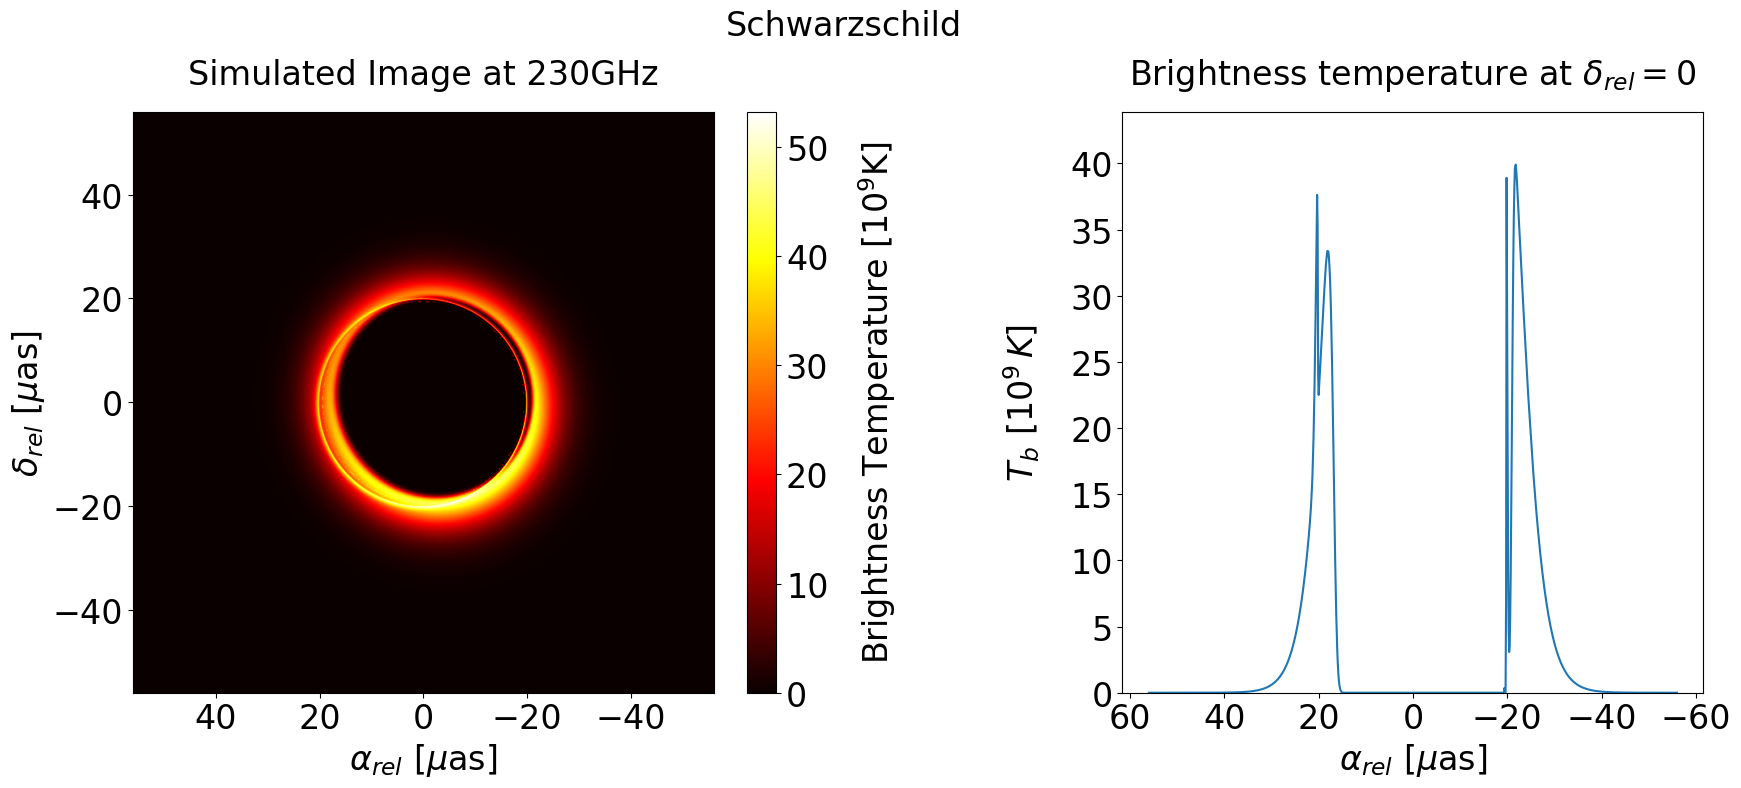
\includegraphics[scale = 0.3]{Ray_tracer_plot_230_Sch.png}
	\end{subfigure}\\
	\begin{subfigure}{12cm}
		\hspace{-1cm}
		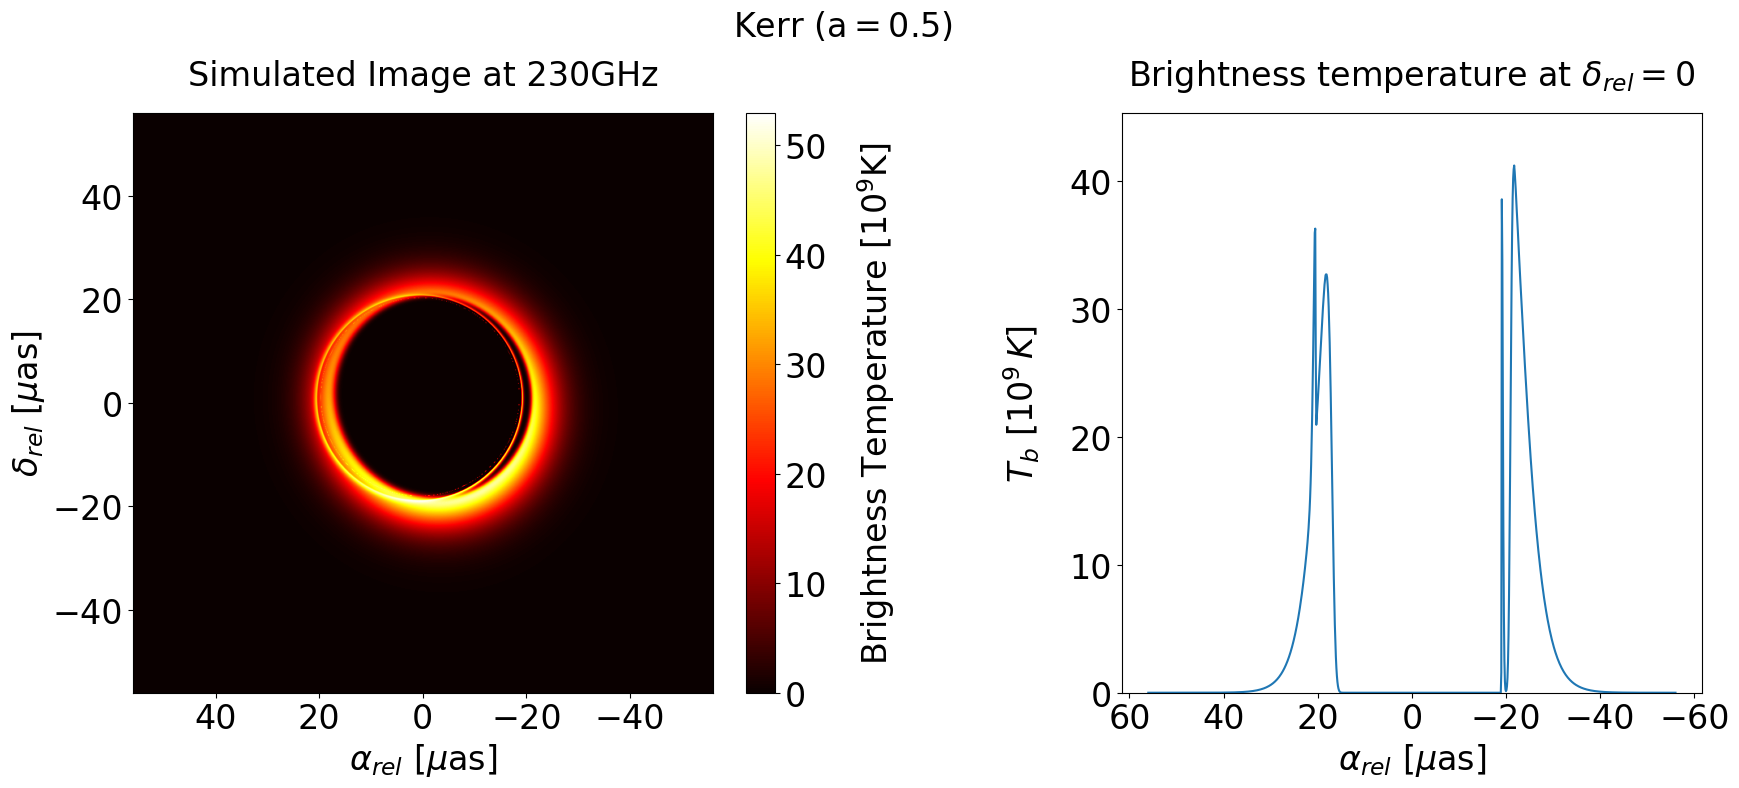
\includegraphics[scale = 0.3]{Ray_tracer_plot_230_Kerr_0.5.png}
	\end{subfigure}\\
	\label{Kerr_Ray_tracer_230}
	\caption[Идеални образи на черни дупки на Кер с реалистичен модел на излъчващата среда, при различен параметър на въртене $a$, и наблюдателна честота $\nu_\text{obs} = 230$ GHz]{\small Идеални образи на черни дупки на Кер с реалистичен модел на излъчващата среда, при различен параметър на въртене $a = \{0, 0.5\}$ и наблюдателна честота $\nu_\text{obs} = 230$ GHz. Температурата при $r = r_0,\,\,\theta = \frac{\pi}{2}$ за двете симулации е фиксирана на $T_0 = 6.8\times10^{10}$ K и $r_0 = 4.5M$. Пълният поток е $\mathcal{F}_{\text{tot}} = 0.574$ Jy за Шварцшилд, и $\mathcal{F}_{\text{tot}} = 0.582$ Jy за Кер. За останалите параметри виж таблица \ref{table:Common_ray_tracer_params}.} 
\end{figure}

Разглеждаме ефекта на въртенето, като извършваме симулации при стойности на параметъра на въртене $a = \{0, 0.5\}$. Резултатите са показани на фигура 8.1, където също сме начертали сечение на яркостната температура през правата $\delta_{\text{rel}} = 0$ на образите, докато на фигура 8.2 (и 8.11 за наблюдателна честота 345 GHz) са представени резултатите за гола сингулярност на Гаус-Боне и на Джанис-Нюман-Уиникър за избрани стойности на параметрите $\gamma$ в метриките им.\\

\noindent Виждаме, че интензитетът на централните образи е значителен. Той представлява максималният за целият образ на Джанис-Нюман-Уиникър, а за Гаус-Боне е само леко занижен, спрямо този на директният образ. Дори и оптическото разделяне на тези образи от EHT да е трудно, значителният поток от централните образи би се отразил върху реконструкцията на образите. В следващите глава оценяваме количествено този ефект.
\newpage

\begin{figure}[h!]
	\centering
	\begin{subfigure}{12cm}
		\hspace{-1cm}
		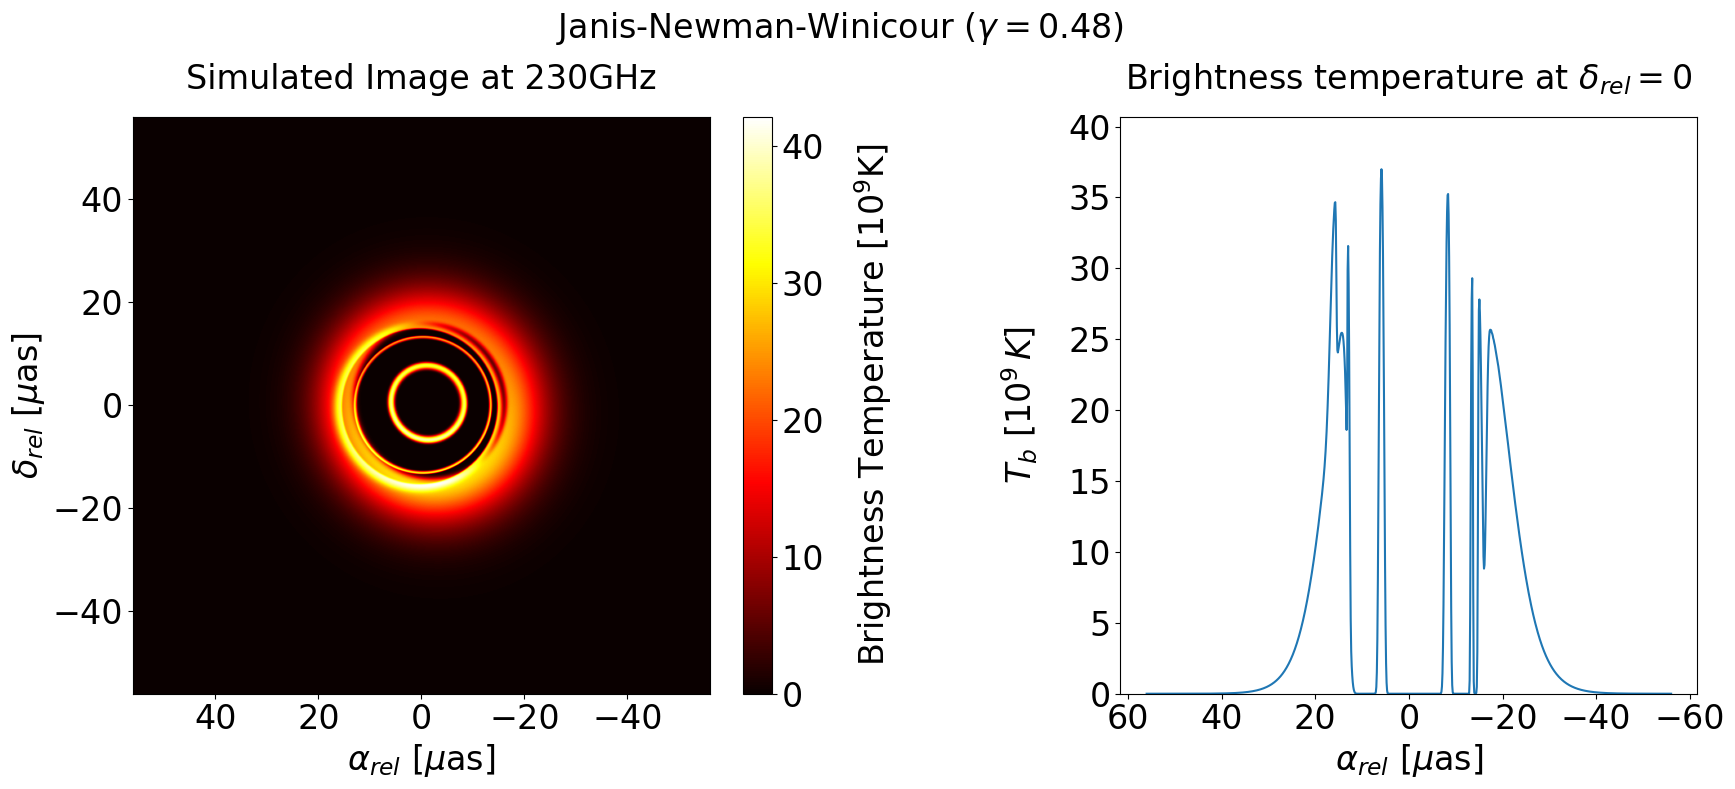
\includegraphics[scale = 0.3]{Ray_tracer_plot_230_JNW.png}
	\end{subfigure}\\
	\begin{subfigure}{12cm}
		\hspace{-1cm}
		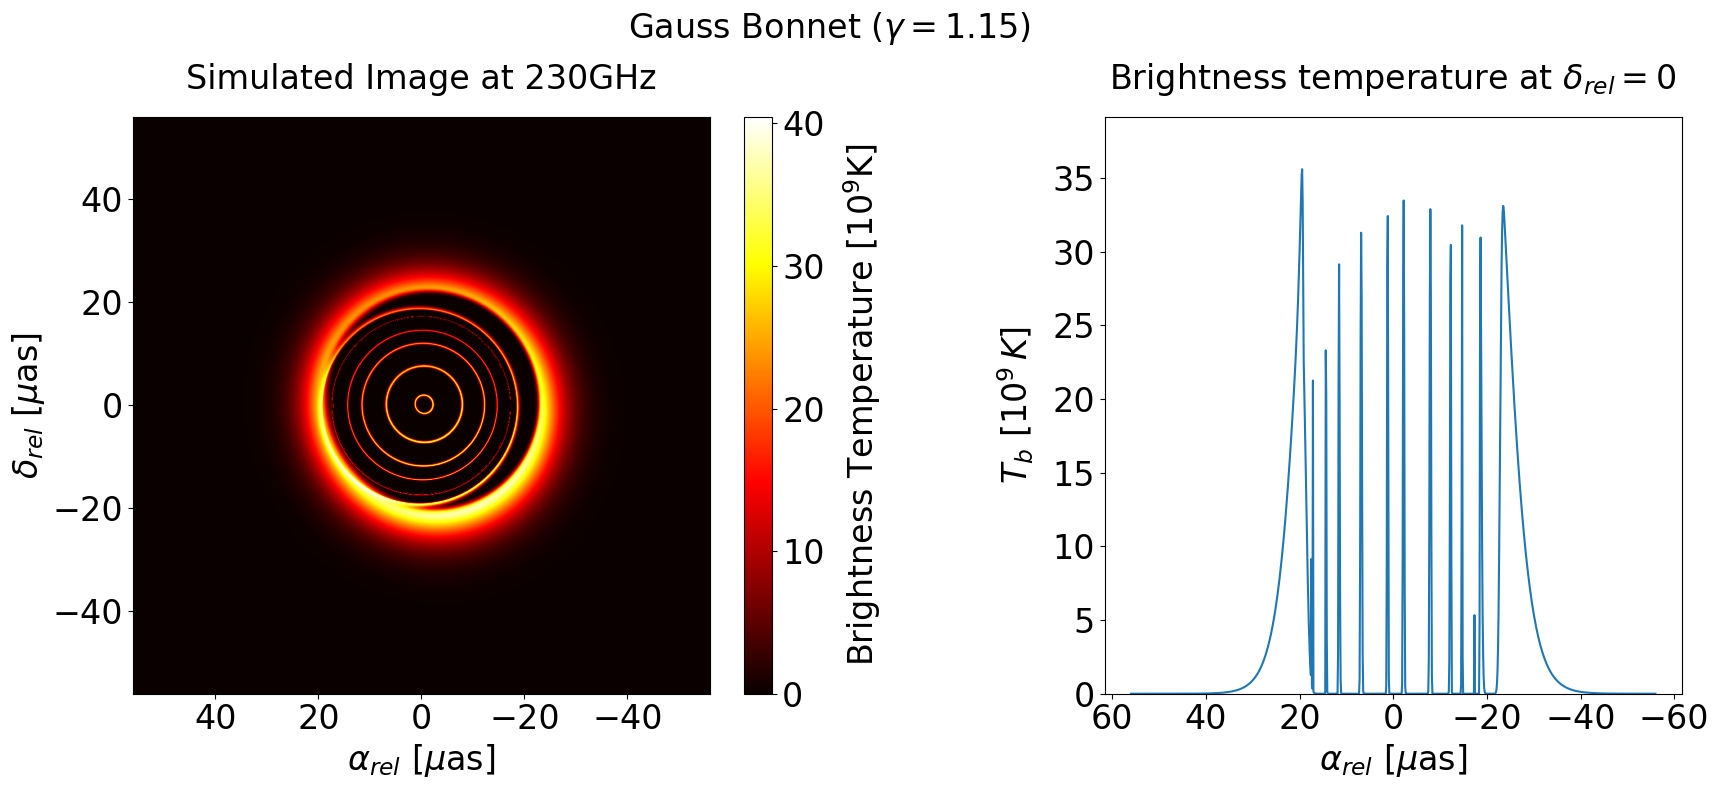
\includegraphics[scale = 0.3]{Ray_tracer_plot_230_GB.png}
	\end{subfigure}\\
	\label{Naked_Singularity_Ray_tracer_230}
	\caption[Идеални образи на голи сингулярности с реалистичен модел на излъчващата среда, при избрани стойности на $\gamma$ и наблюдателна честота $\nu_\text{obs} = 230$ GHz.]{\small Идеални образи на голи сингулярности с реалистичен модел на излъчващата среда, при избрани стойности на $\gamma$ и наблюдателна честота $\nu_\text{obs} = 230$ GHz6. Температурата при $r = r_0,\,\,\theta = \frac{\pi}{2}$ за Джанис-Нюман-Уиникър е $T_0 = 7.2\times10^{10}$ K, докато за Гаус-Боне е $T_0 = 5.9\times10^{10}$. Пълният поток е съответно $\mathcal{F}_{\text{tot}} = 0.574$ Jy и $\mathcal{F}_{\text{tot}} = 0.582$ Jy. Параметърът $r_0$ е фиксиран на $r_0 = 5M$ за двете решения. За останалите параметри виж таблица \ref{table:Common_ray_tracer_params}.} 
\end{figure}


\subsection{Реконструкция на образите}

Както вече споменахме, използваме библиотеката ehtim$^{18}$ за реконструцията на образите на компактните обекти от фигура 8.1 и 8.2. Методиката зад реконструциите е обсъдена в \cite{EHTIM}. Тук само ще обобщим използваните настройки на ehtim - параметрите на симулираното наблюдение, и тези на алгоритъма за реконструкция. След това ще коментираме получените резултати.\\

Разглеждаме 3 конфигурации на телескопи - тази от кампанията от 2017 г., 2022г. и преспективна конфигурация за бъдещи наблюдения, наричана ngEHT. Първите две наблюдават единствено на честота $230$ GHz, докато ngEHT наблюдава на $230$ GHz и 345 GHz. Физическите параметри на самите телескопи са дадени в таблица в \cite{Deliyski2024}. \\

Първо използваме пакета ehtim за да генерираме т.н. \emph{синтетично наблюдение}. То представлява симулация на $(u,v)$ покритието при реално наблюдение и има следните входни параметри: време на интеграция $\Delta t$, време между интегрирания $T$, продължителност на наблюдението $T_\text{obs}$ и широчина на честотната лента $\Delta\nu$. Избраните от нас параметри са съобразени с \cite{EHTIM}, и са дадени в таблица \ref{table:ehtim_obs_settings}.\\

\begin{minipage}{18em}
	\begin{center}
		\begin{tabular}{|| m{7.5em} | m{5em} | m{2em} ||}
			\hline 
			Конфигурация от телескопи & \multicolumn{2}{m{7em}||}{Параметри на синтетичните наблюдения} \\
			\hline
			\multirow{4}{7.5em}{\centering \small EHT 2017 / 2022} &\centering $\Delta t,\, [s]$    		& 5   \\ 
														&\centering $T,\,[s]$ 		     		& 30  \\ 
														&\centering $T_\text{obs},\,[h]$ 		& 24  \\
														&\centering $\Delta \nu,\,[\text{GHz}]$ & 4 \\
			\hline
			\multirow{4}{7.5em}{\centering \small ngEHT} 		  & \centering $\Delta t,\, [s]$    	   & 120 \\ 
													  & \centering $T,\,[s]$ 		      	   & 600 \\ 
												      & \centering $T_\text{obs},\,[h]$ 	   & 24  \\
												      & \centering $\Delta \nu,\,[\text{GHz}]$ & 2 \\
			\hline
		\end{tabular}
	\end{center}
	\captionof{table}[Настройки на синтетичните наблюдения.]{Настройки на синтетичните наблюдения.}
	\label{table:ehtim_obs_settings}
\end{minipage}\,\,
\begin{minipage}{18em}
	За настройките на алгоритъма за реконструкция следваме \cite{EHTIM}. Избираме да работим с два члена $\chi^2(I,d)$ члена: $\chi^2_\text{amp}$ и $\chi^2_\text{cl. phase}$. Избираме също така четири регуляризатора: $S_\text{entropy}$, $S_\text{TSV}$, $S_\text{tot flux}$ и $S_\text{centroid}$. Стойностите на хиперпараметрите $\alpha_D$ и $\beta_R$, както и броя стадии и итерации на алгоритъма, са обобщени в таблица \ref{table:reconstruction_settings}. С цел увеличаване на сходимостта на алгоритъма, правим конвулюция на полученото изображение след всеки стадии с Гаусов сигнал, имащ стандартно отклонение $\sigma = f_\text{blur} \sigma_{\text{230 GHz}}$, където $\sigma_{\text{230 GHz}}$ е номиналната резолюция на цялата конфигурация от телескопи при 230 GHz.
\end{minipage}

\begin{table}[h!]
	\centering
	\begin{tabular}{||c|c|c|c|c|c|c|c|c||}
		\hline
		\hline
		\thead{ Стадии } & \thead{$f_\text{blur}$} &\thead{$\beta_\text{entropy}$} &\thead{$\beta_\text{TSV}$} &\thead{$\beta_\text{tot flux}$} & $\beta_\text{centroid}$
						 & \thead{$\alpha_\text{amp}$} & \thead{$\alpha_{\text{cl. phase}}$} & $N_\text{iter}$\\
		\hline
		\thead{1}  &  \thead{NA} & \thead{1} &\thead{1} &\thead{100} & \thead{100} &\thead{100} &\thead{200} &\thead{1000} \\  
		\hline
		
		\thead{2}  &  \thead{0.75} & \thead{1} &\thead{50} &\thead{50} & \thead{50} &\thead{100} &\thead{75} &\thead{3000} \\  
		\hline
		
		\thead{3}  &  \thead{0.5} & \thead{1} &\thead{100} &\thead{10} & \thead{10} &\thead{100} &\thead{50} &\thead{4000} \\  
		\hline
		
		\thead{4}  &  \thead{0.33} & \thead{1} &\thead{500} &\thead{1} & \thead{1} &\thead{100} &\thead{100} &\thead{4000} \\  
		\hline
		\hline

	\end{tabular}
	\caption[Параметри на алгоритъма за реконструкция.]{Параметри на алгоритъма за реконструкция.}
	\label{table:reconstruction_settings}
\end{table}

Финалното изображение отново конвулираме с Гаусов сигнал, имащ $\sigma = \sigma_\text{clean} / 2$, където $\sigma_\text{clean}$ е стандартното отклонение на "чистия сноп". Това се прави понеже в противен случай алгоритъма би произвел изображение с резолюция, много по-голяма от тази на самите телескопи.\\
\newpage
\subsubsection{Реконструкция от EHT 2017 / 2022}

На фигури 8.3 и 8.4 показваме реконструкциите на образите, получени от симулациите, показани на фигури 8.1 и 8.2. За всеки реконструиран образ даваме получените стойности за функциите $\chi^2_\text{amp}$ и $\chi^2_\text{cl. phase}$. Получаваме, че реконструкциите от двата набора телескопи EHT 2017 и EHT 2022 са изключително сходни, и затова избираме да покажем само тези от EHT 2017 (с изключение на голата сингулярност на Джанис-Нюман-Уиникър, показана на фигура 8.5), но количествения анализ в подточка 8.4 ще бъде представен и за двете конфигурации.


\begin{figure}[h!]
	\centering
	\begin{subfigure}{12cm}
		\hspace{-1.5cm}
		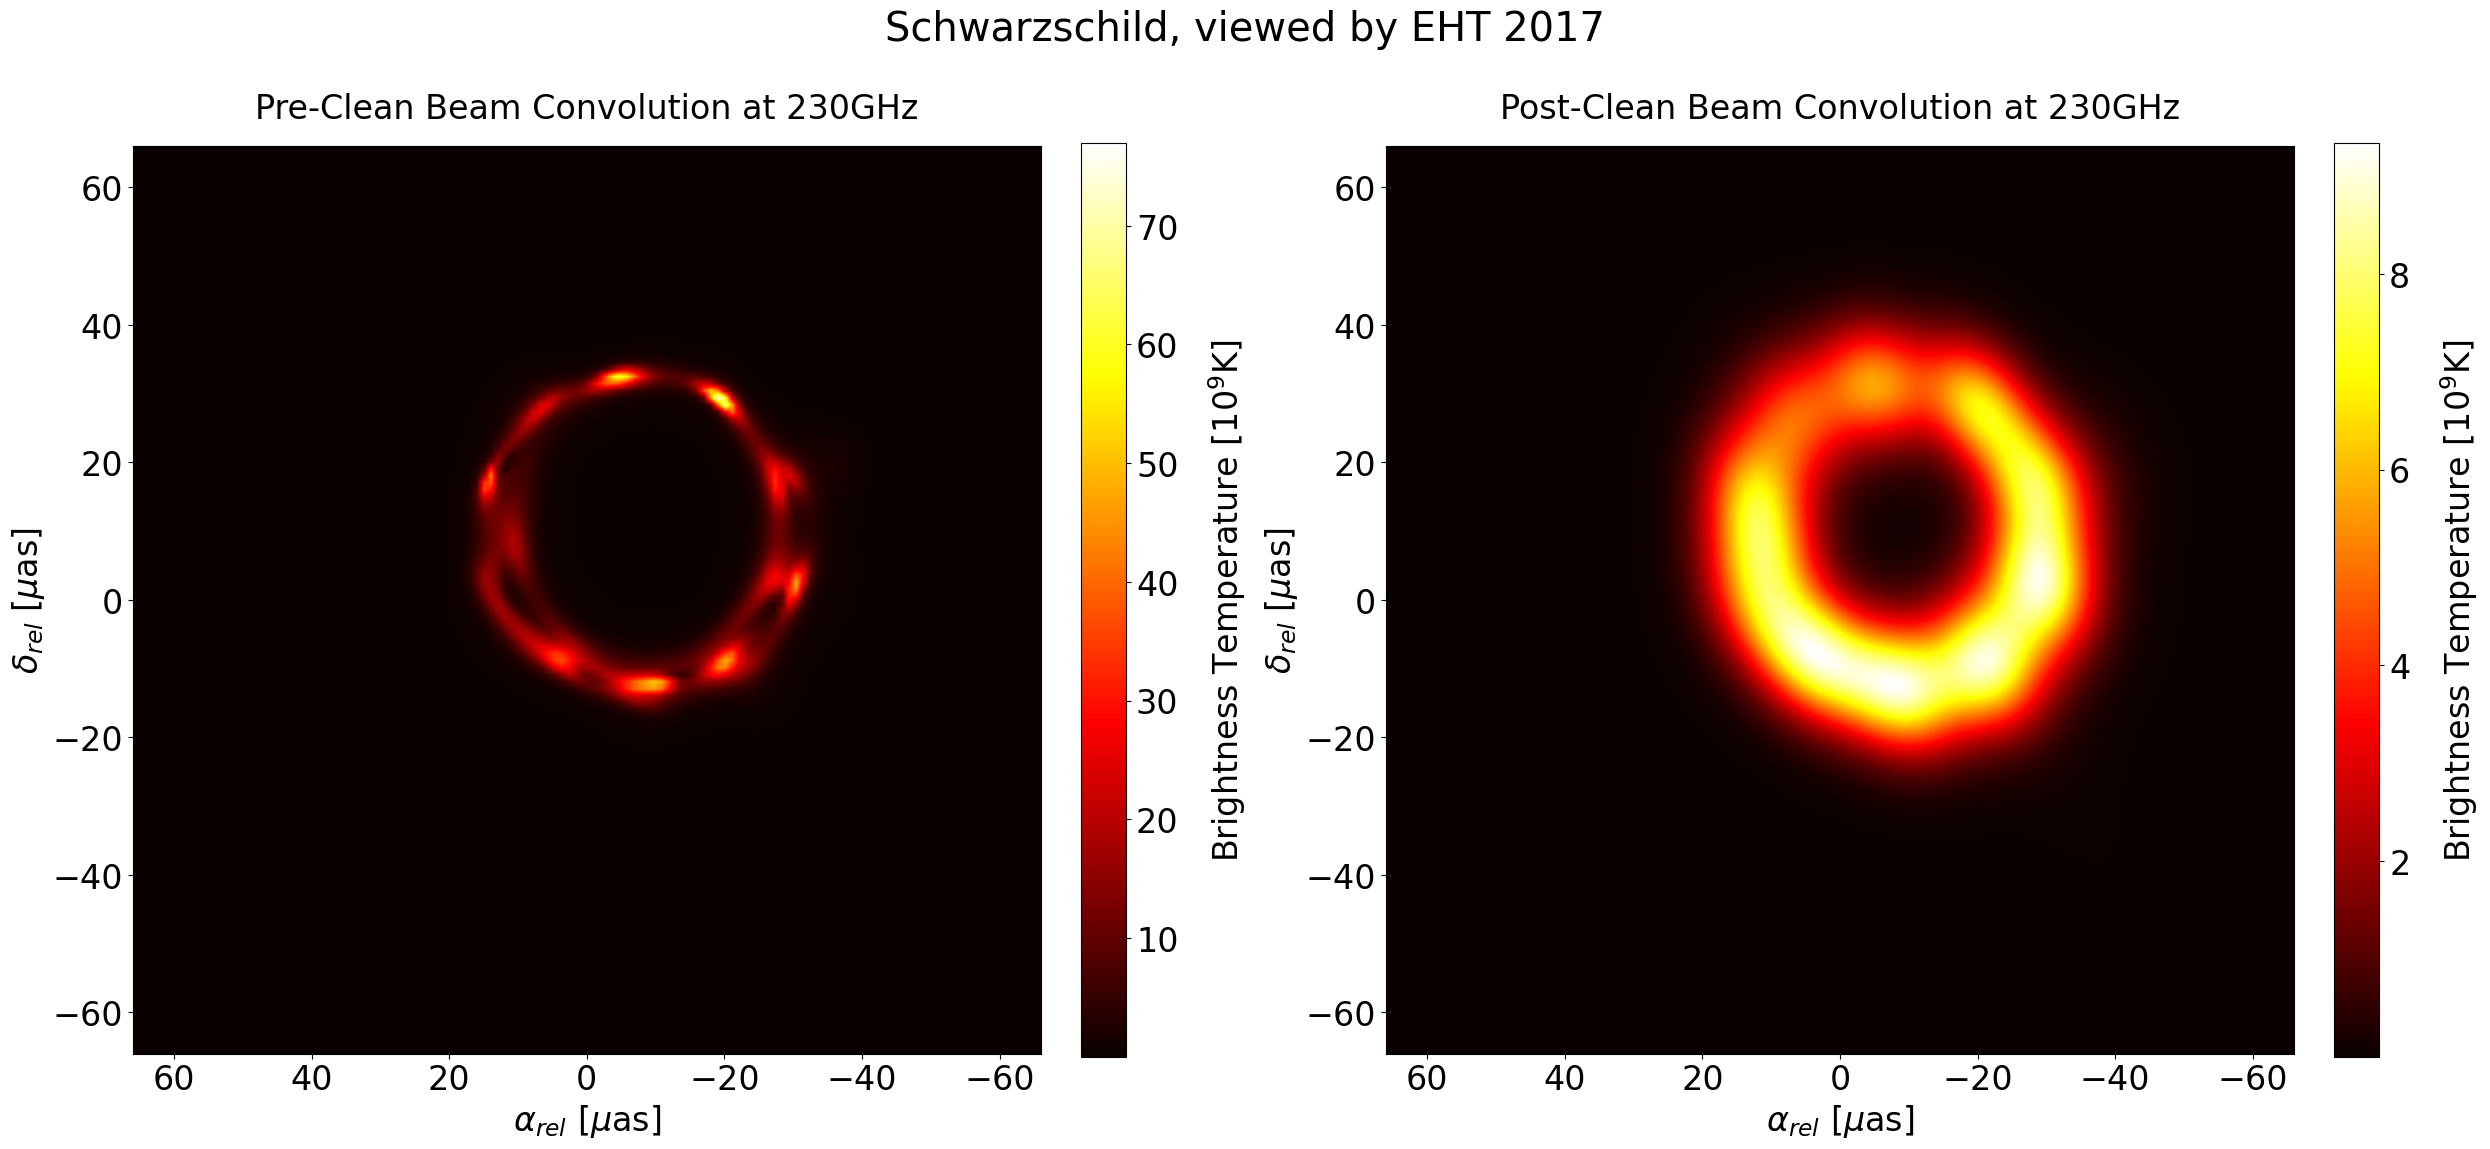
\includegraphics[scale = 0.23]{Ehtim_plot_2017_no_blur_Sch.png}
	\end{subfigure}\\
	\begin{subfigure}{12cm}
		\hspace{-1.5cm}
		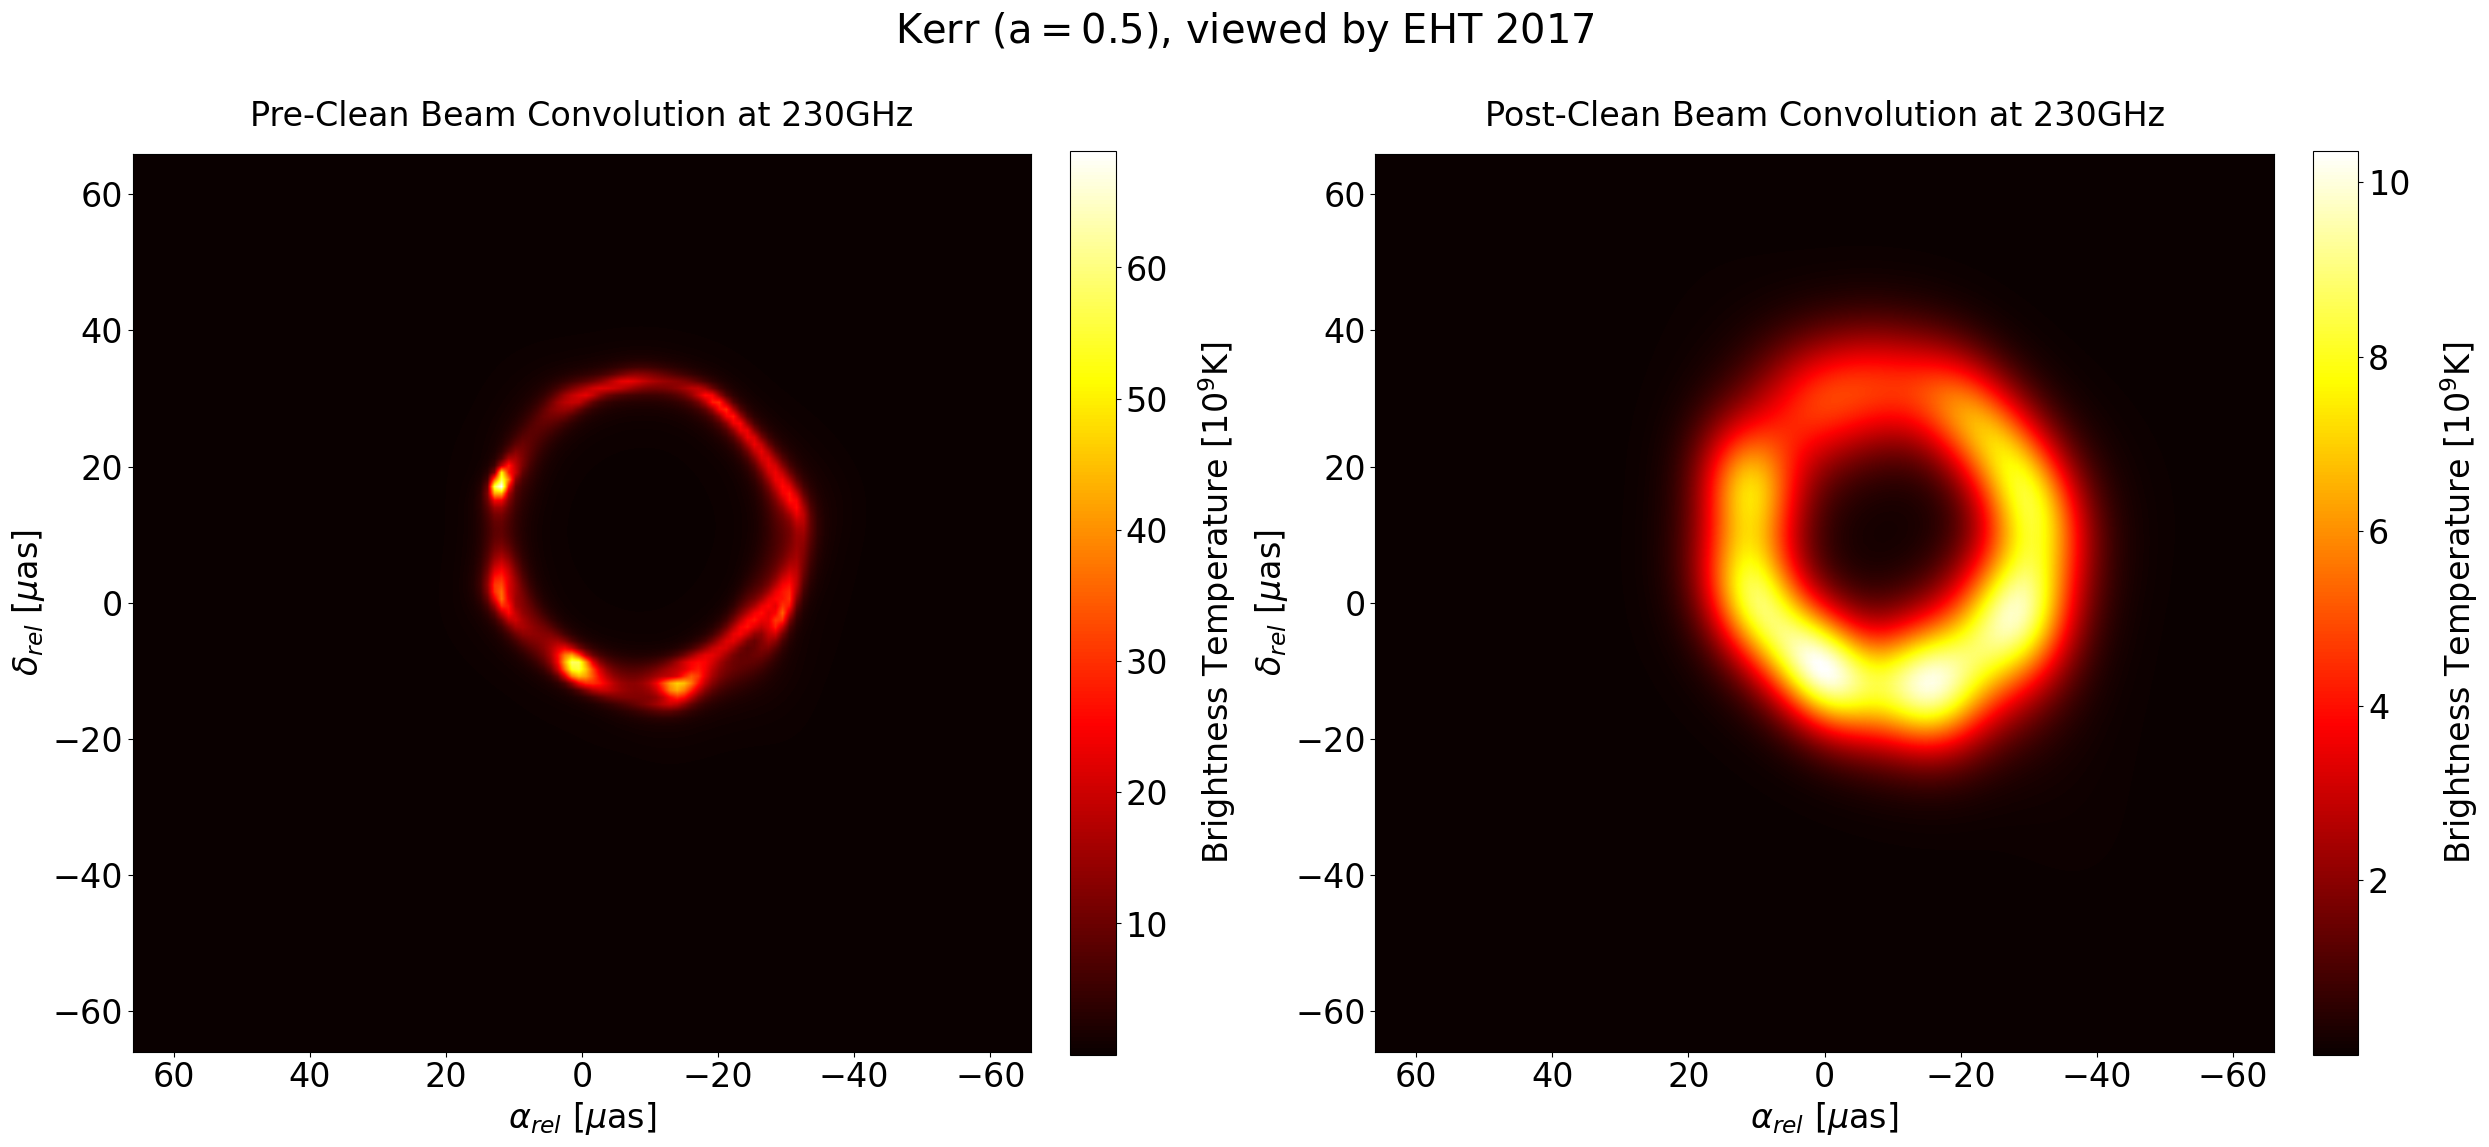
\includegraphics[scale = 0.23]{Ehtim_plot_2017_no_blur_Kerr.png}
	\end{subfigure}\\
	\label{Kerr_EHT_2017}
	\caption[Реконструирани образи на черни дупки на Кер при различни параметри на въртене.]{\small Реконструирани образи на черни дупки на Кер при различни параметри на въртене $a = \{0, 0.5\}$. Левият панел показва "голата"$\,$ реконструкция, преди коволюцията с "чистия сноп". Финалните стойности на $\chi^2$ са $\chi^2_\text{amp} = \{1.02, 1.04\}$ и $\chi^2_\text{cl. phase} = \{0.9, 1.07\}$ за $a = \{0, 0.5\}$.} 
\end{figure}

\newpage

Виждаме от фигура 8.4, че ефективната резолюция на набора телескопи не е достатъчно висока при $230$ GHz за да различи наличието на екзотичните образи. Те се "размиват"$\,$ и сливат с останалите. Забелязваме обаче, че това води до значително повишен поток в централната депресия. Можем да оценим количествено потока от този регион и да дефинираме с това мярка, по която да съдим за наличието на екзотични образи. 


\begin{figure}[h!]
	\centering
	\begin{subfigure}{12cm}
		\hspace{-1.5cm}
		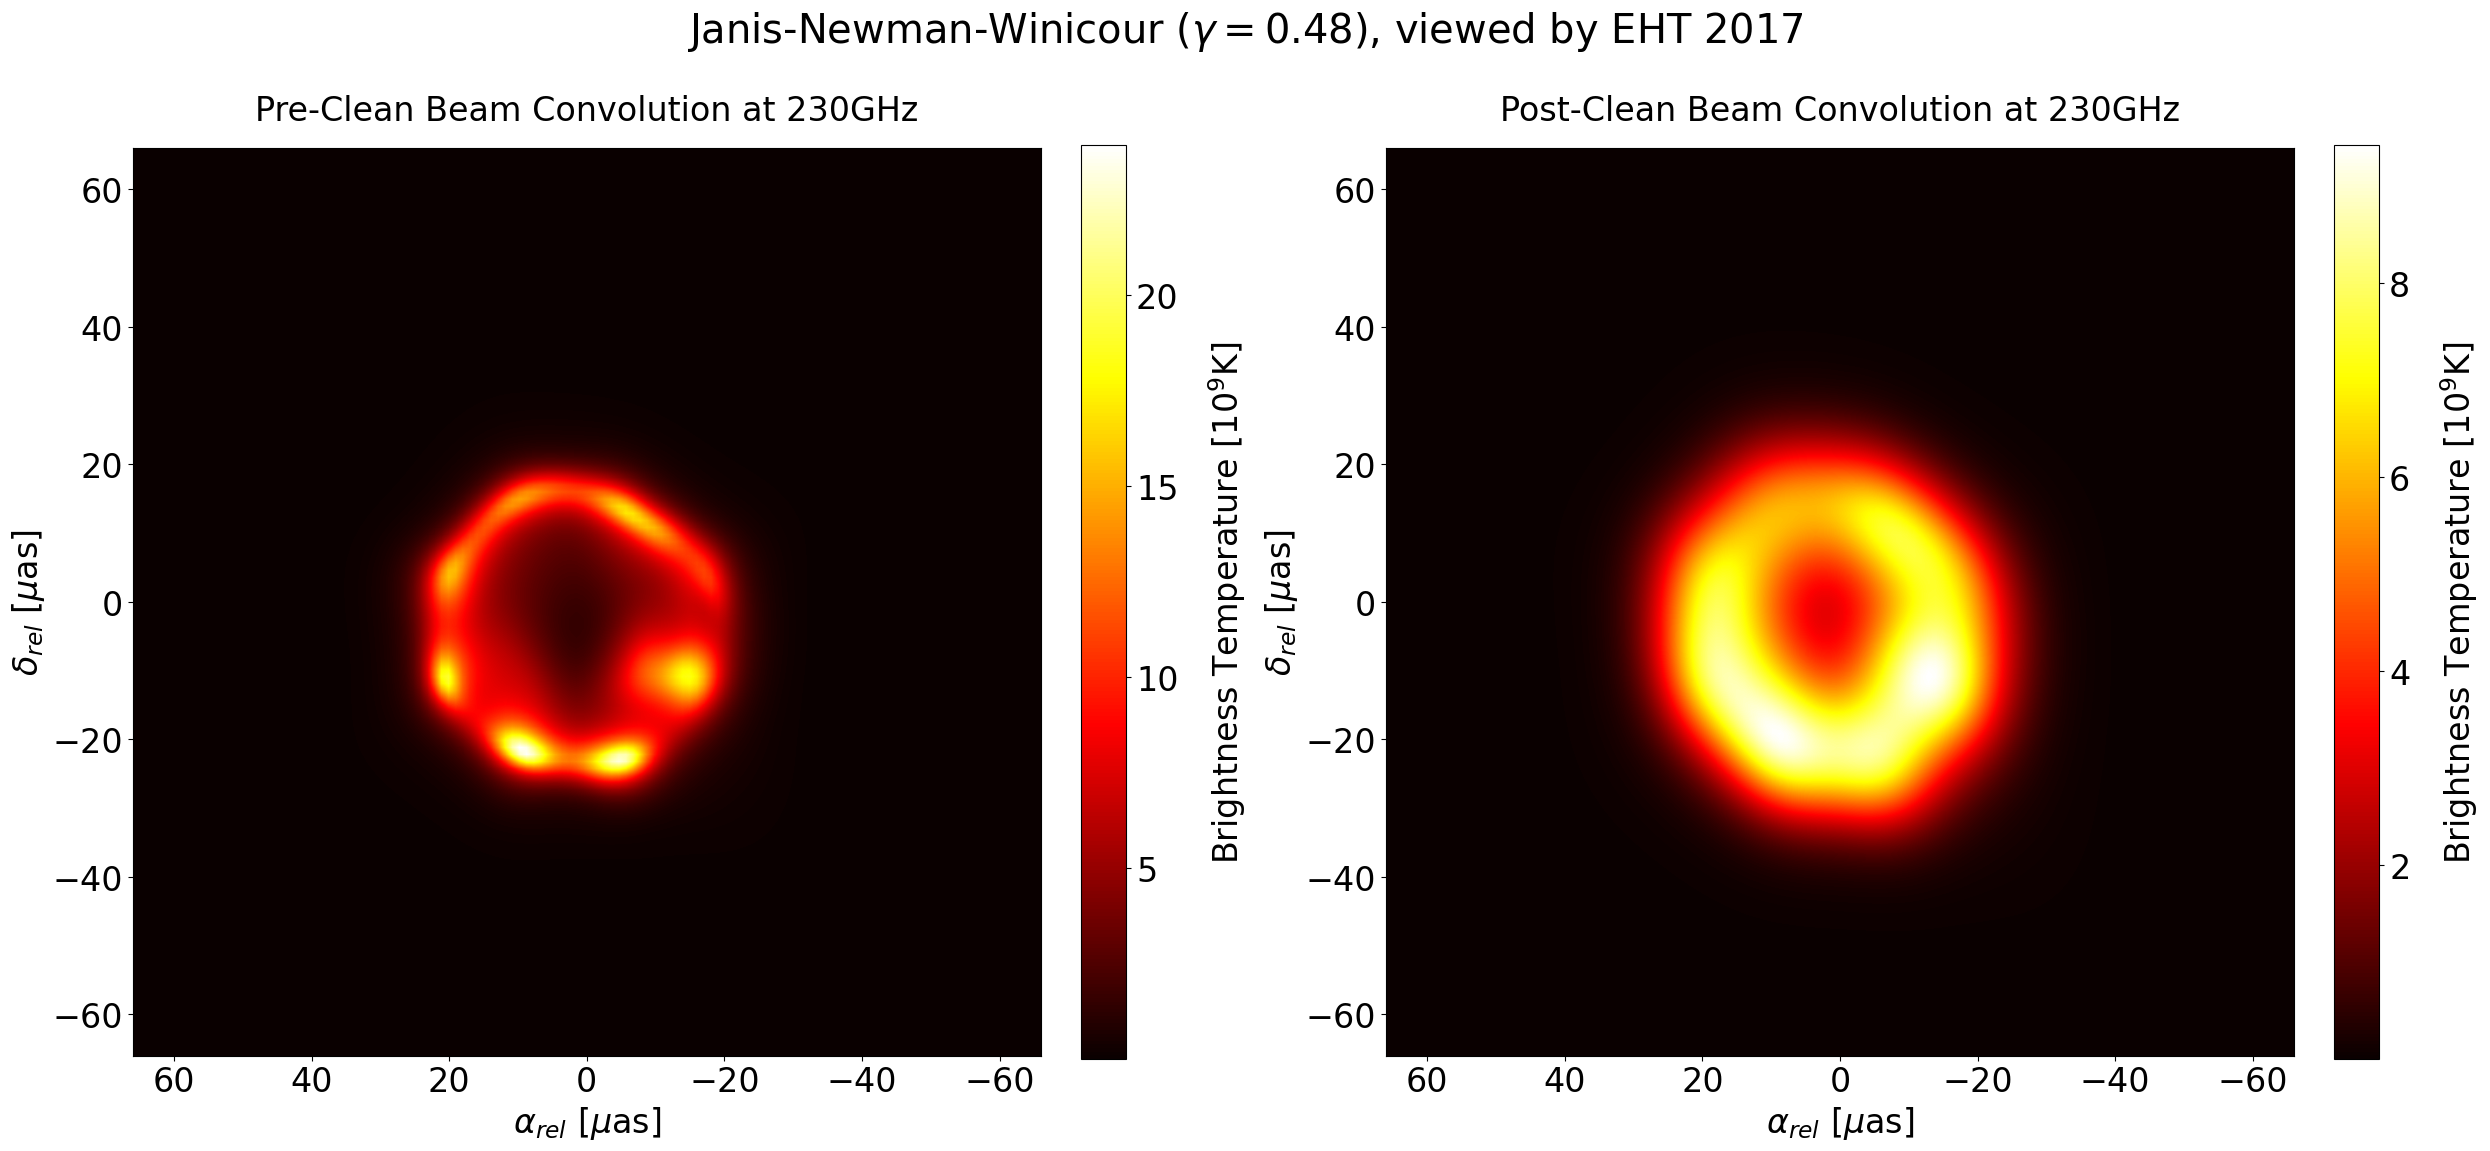
\includegraphics[scale = 0.23]{Ehtim_plot_2017_no_blur_JNW.png}
	\end{subfigure}\\
	\begin{subfigure}{12cm}
		\hspace{-1.5cm}
		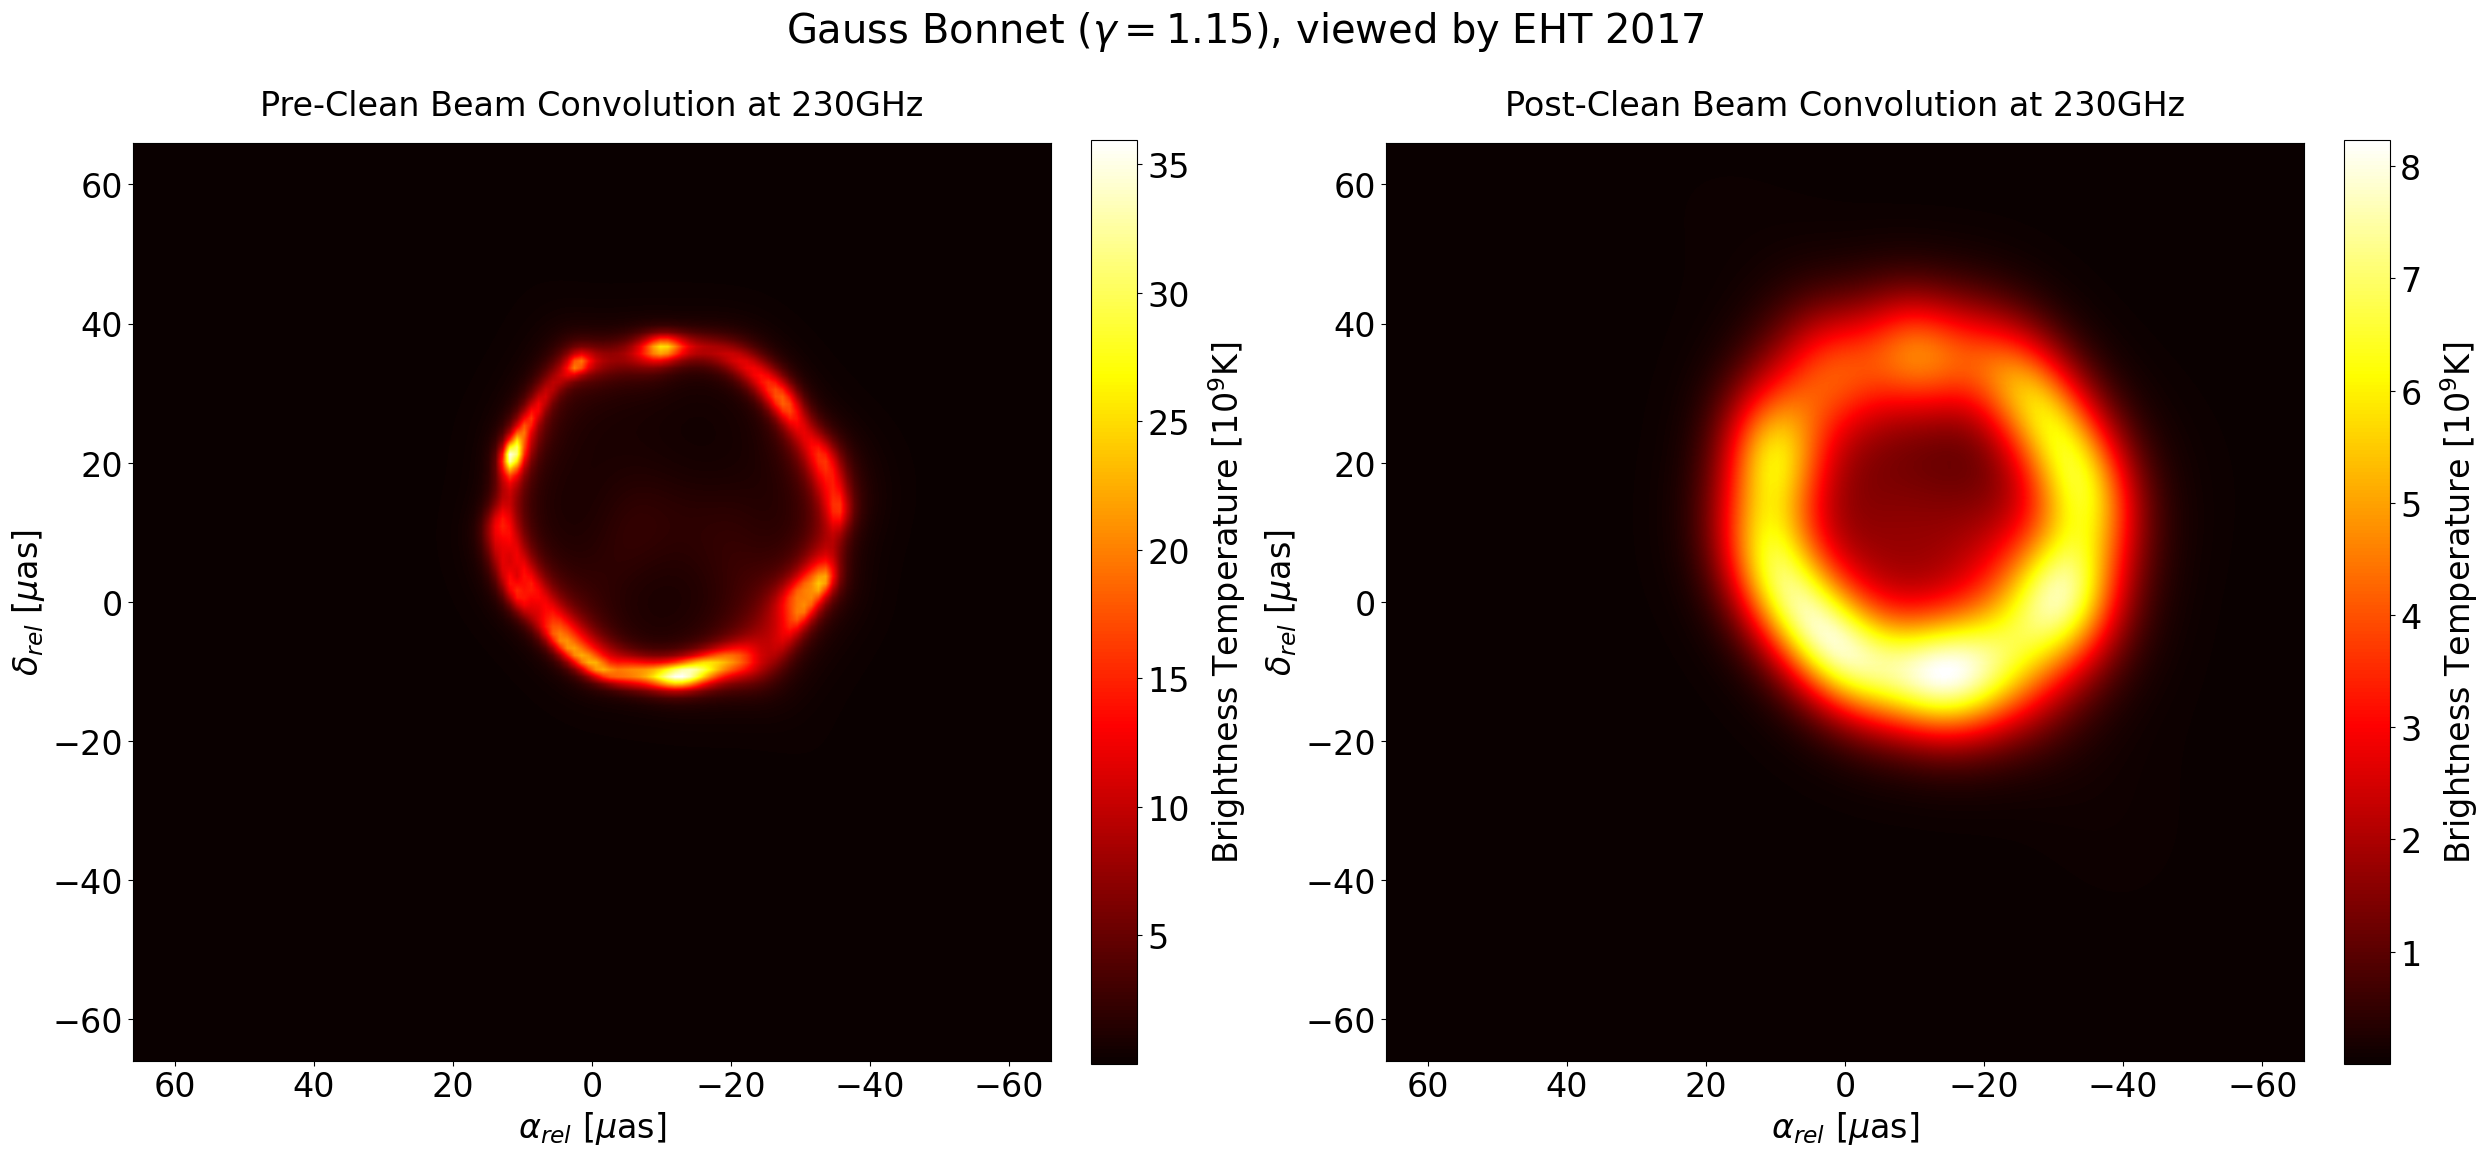
\includegraphics[scale = 0.23]{Ehtim_plot_2017_no_blur_GB.png}
	\end{subfigure}\\
	\label{Naked_Singularity_EHT_2017}
	\caption[Реконструирани образи на голи сингулярности, при избрани стойности на $\gamma$, от EHT 2017]{\small Реконструирани образи на голи сингулярности, при избрани стойности на $\gamma$, от EHT 2017. Левият панел показва "голата"$\,$ реконструкция, преди коволюцията с "чистия сноп". Финалните стойности на $\chi^2$ са $\chi^2_\text{amp} = \{1.01, 1.00\}$ и $\chi^2_\text{cl. phase} = \{0.91, 0.84\}$ съответно за Гаус-Боне и Джанис-Нюман-Уиникър.} 
\end{figure}

\begin{figure}[h!]
	\centering
	\begin{subfigure}{6cm}
		\hspace{-1.5cm}
		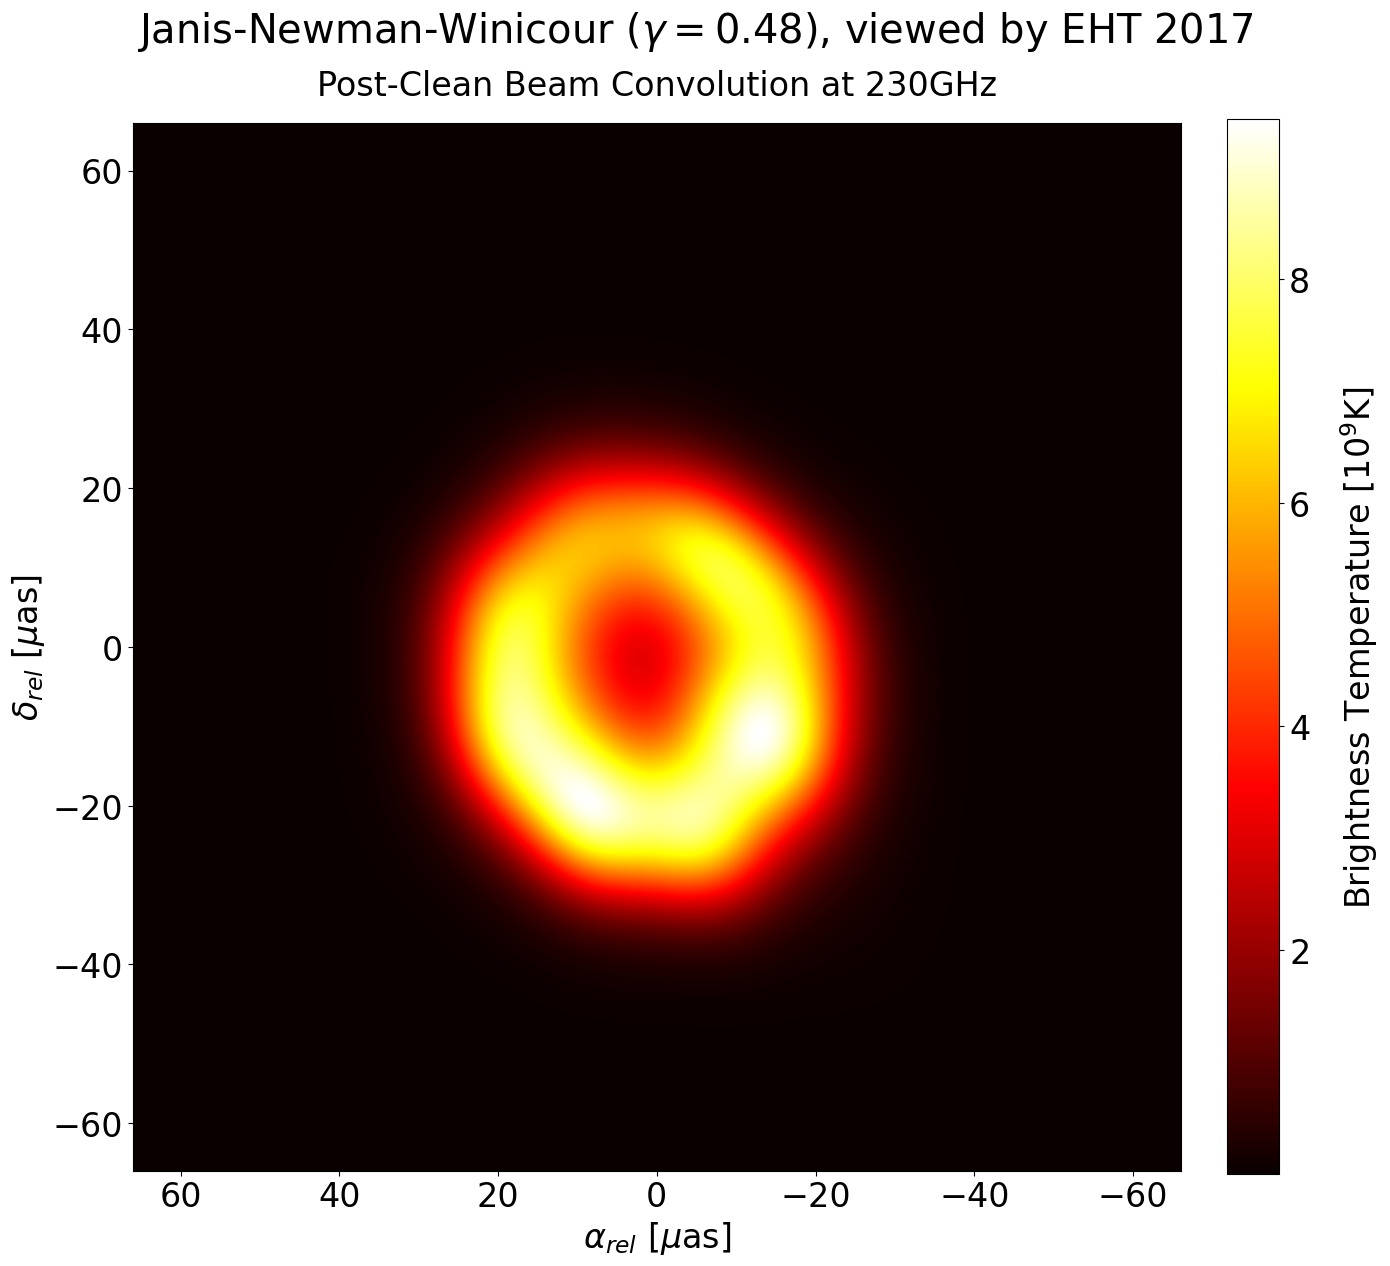
\includegraphics[scale = 0.20]{Ehtim_plot_2017_JNW.png}
	\end{subfigure}
	\begin{subfigure}{6cm}
		\hspace{-0.0cm}
		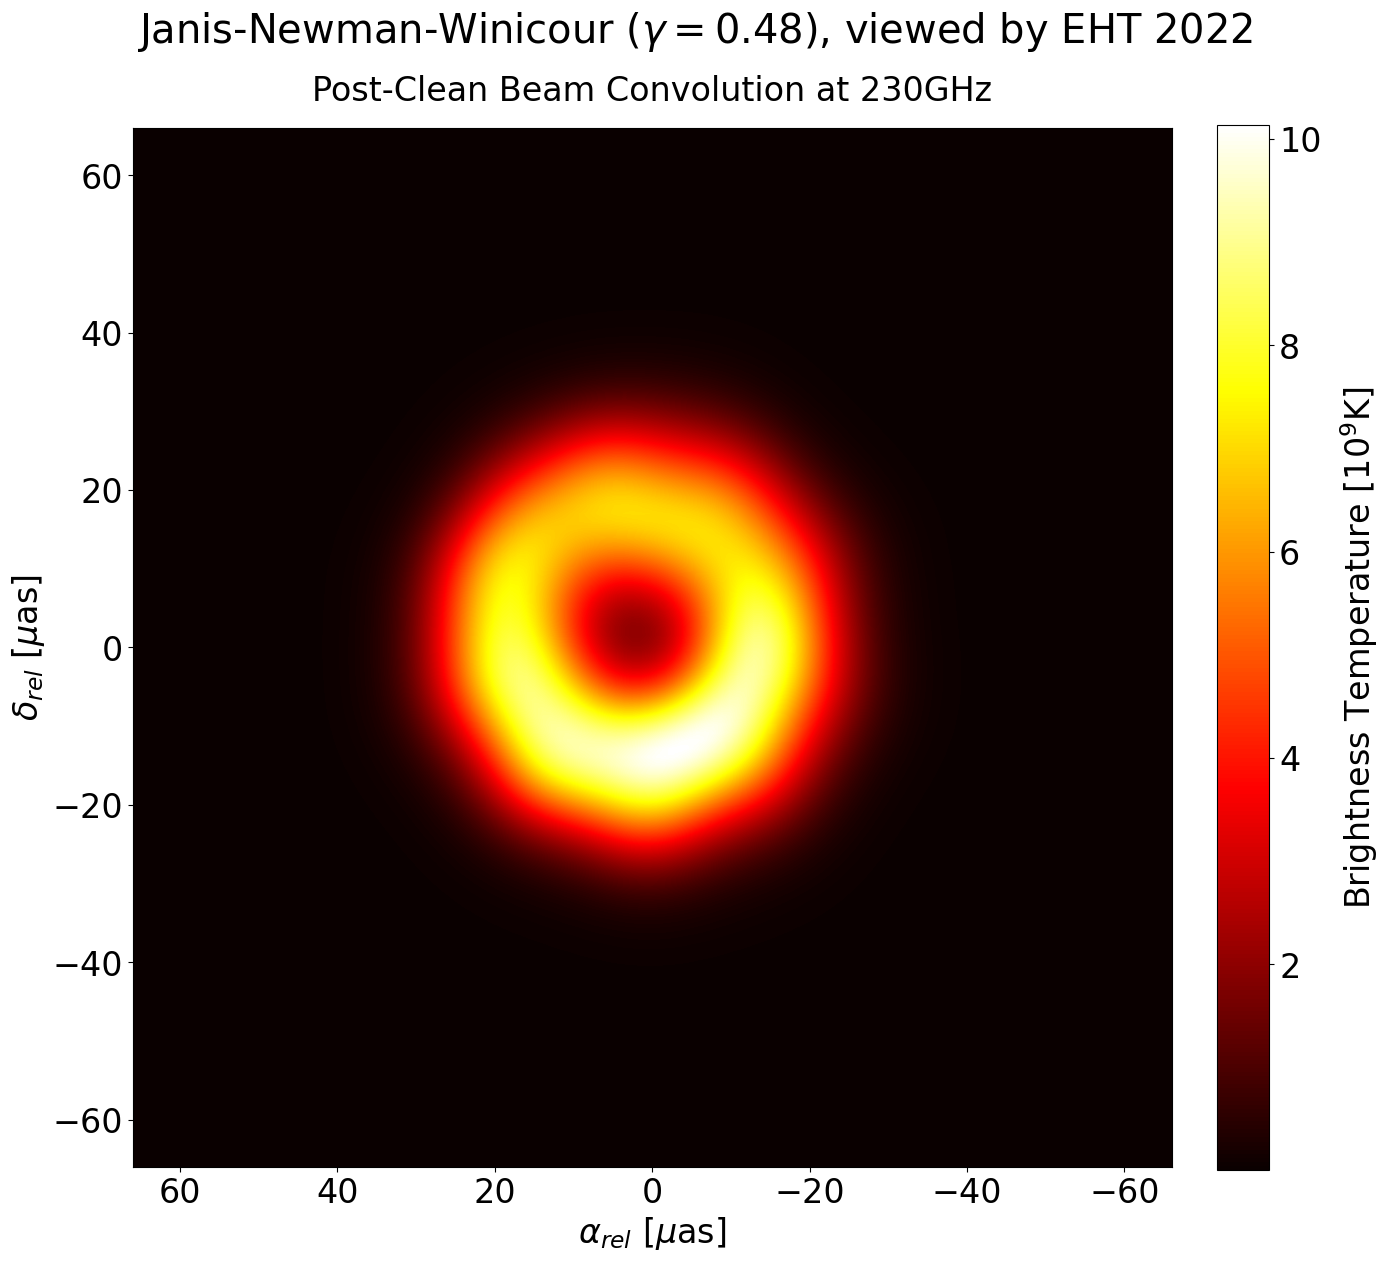
\includegraphics[scale = 0.20]{Ehtim_plot_2022_JNW.png}
	\end{subfigure}
	\label{EHTIM_JNW_2017_2022}
	\caption[Сравнение между реконструкциите от EHT 2017 и EHT 2022 на голата сингуларност на Джанис-Нюман-Уиникър]{Сравнение между реконструкциите от EHT 2017 и EHT 2022 на голата сингуларност на Джанис-Нюман-Уиникър. Забелязваме, че EHT 2017 произвежда значително по-елиптичен образ. Също с разширения набор телескопи на EHT 2022, централната депресия е по-добре изразена. Финалните стойности на $\chi^2$ са $\chi^2_\text{amp} = \{1.00, 1.08\}$ и $\chi^2_\text{cl. phase} = \{0.84, 1.01\}$ съответно за EHT 2017 и EHT 2022.} 
\end{figure}

Основното подобрение, което виждаме от разширения набор телескопи за тази конфигурация, е по-ясното изразяване на централна депресия за голата сингуларност на Джанис-Нюман-Уиникър, както и значително по-малка елиптичност на реконструкцията ѝ. Останалите реконструкции са видимо изключително сходни.  
\newpage
\subsubsection{Реконструкция от ngEHT}

Преспективните бъдещи наблюдения на ngEHT освен, че ще включват повече телескопи (тук сме разгледали набор от 21 такива), също ще наблюдават на втора, по-висока честота $\nu = 345$ GHz. По-големият набор от телескопи би подобрил $(u,v)$ покритието, но наличието на втората честота се очаква значително да подобри ефективната резолюция на телескопа. На фигура 8.6 са показани реконструкциите на еквивалента на образите (8.2), но симулирани при $\nu  =345$ GHz. Виждаме, въпреки, че морфология все още не е разделена, наблюденията на 345 GHz вече стават чувствителни към наличието на екзотичните образи. Появява се ясен локален максимум, намиращ се в централната депресия. В следващата подточка ще дадем количествена оценка за тази депресия.

\begin{figure}[h!]
	\centering
	\begin{subfigure}{12cm}
		\hspace{-1.5cm}
		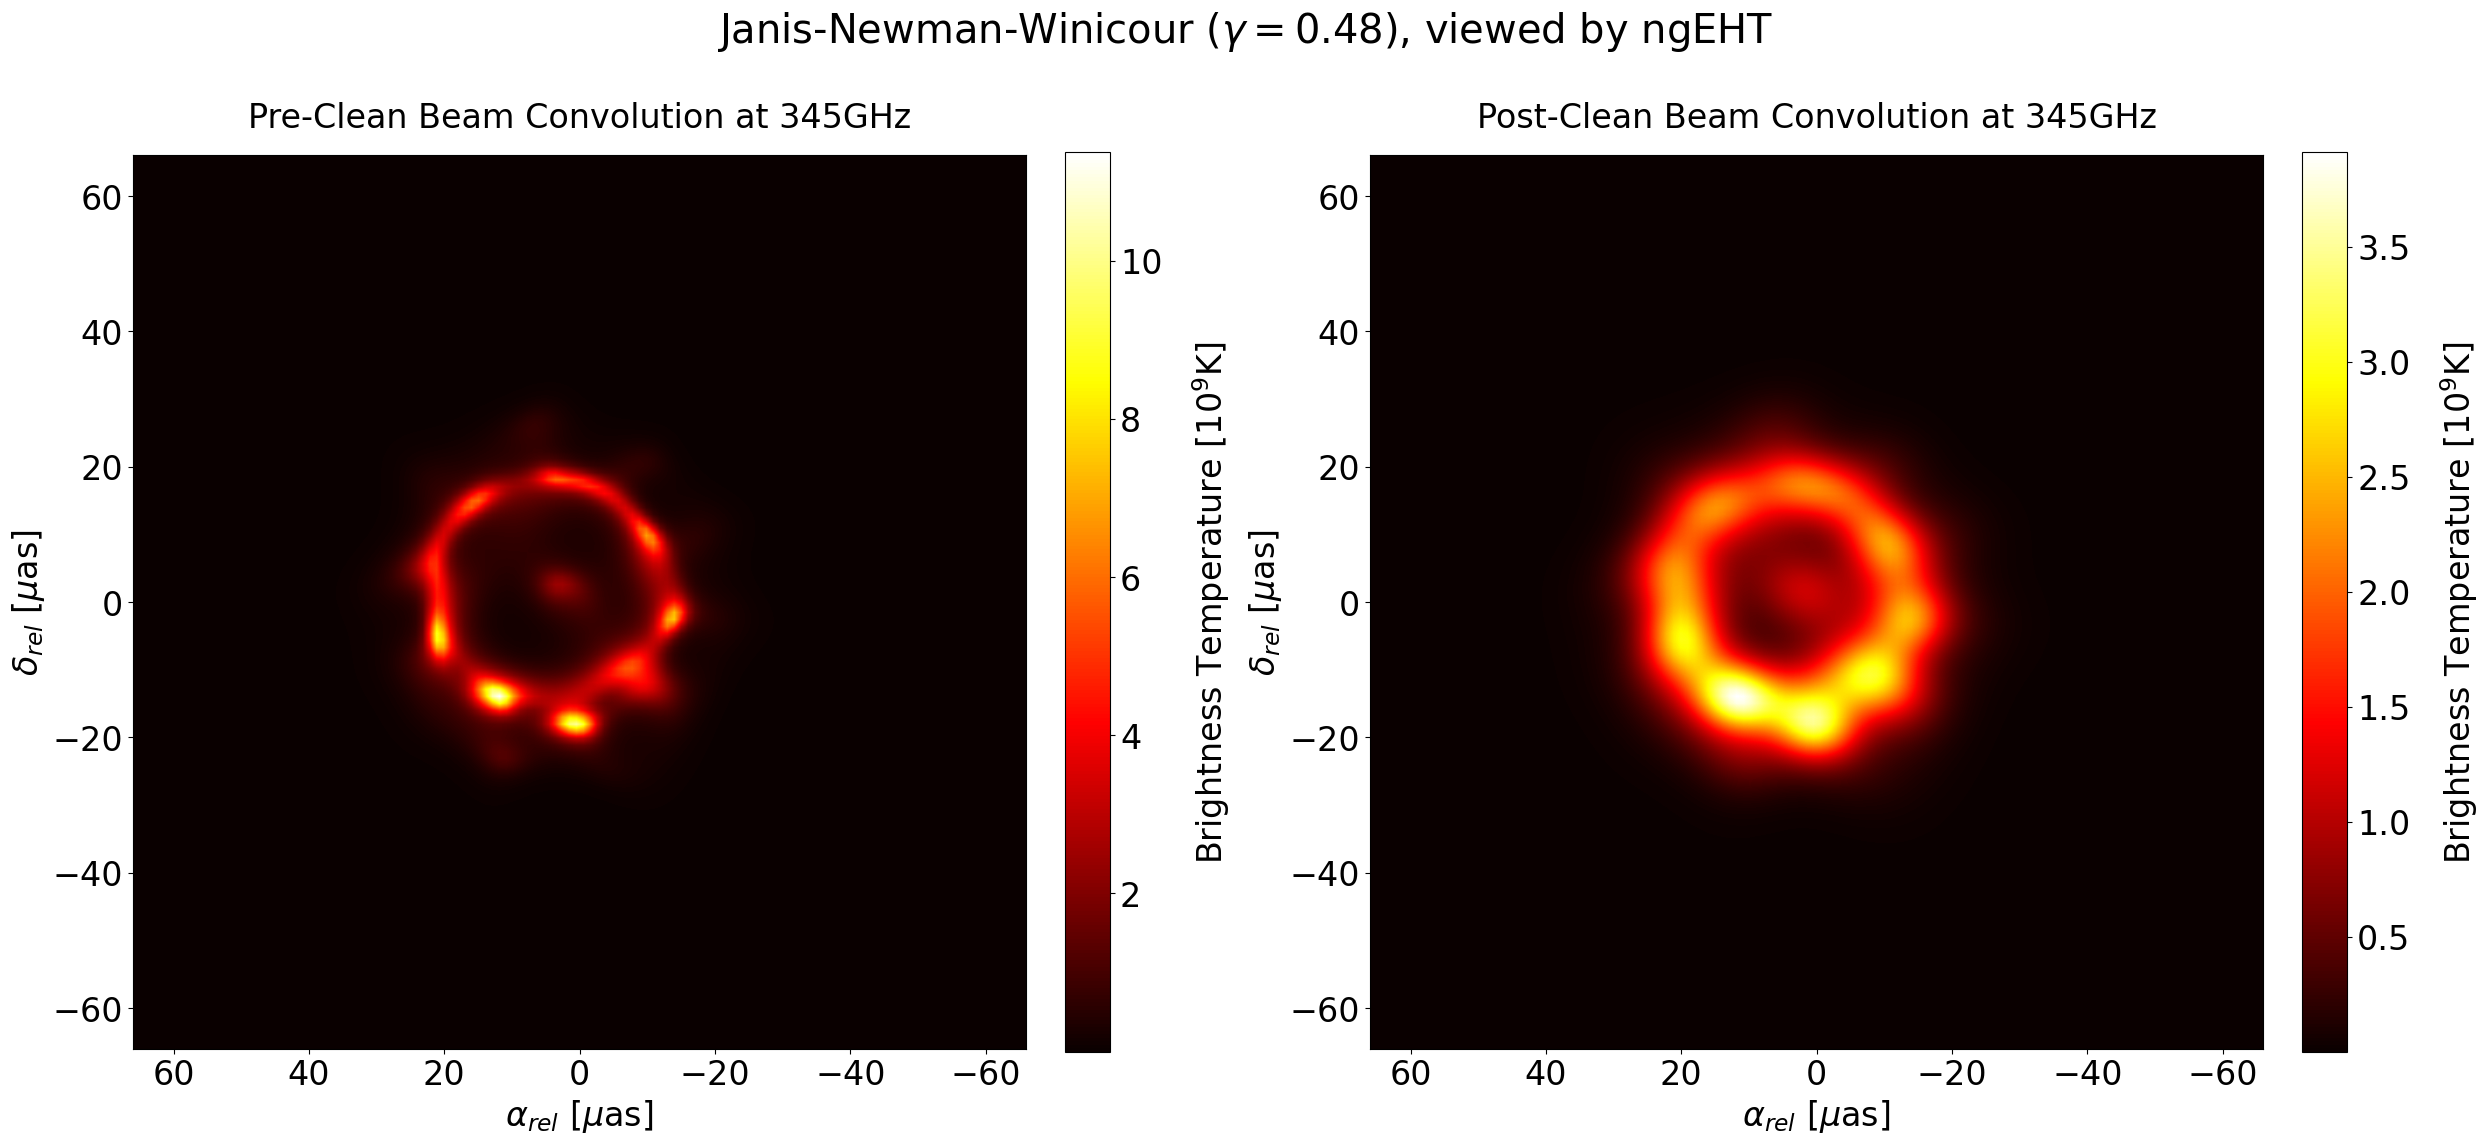
\includegraphics[scale = 0.23]{Ehtim_plot_ngEHT_no_blur_345_JNW.png}
	\end{subfigure}\\
	\begin{subfigure}{12cm}
		\hspace{-1.5cm}
		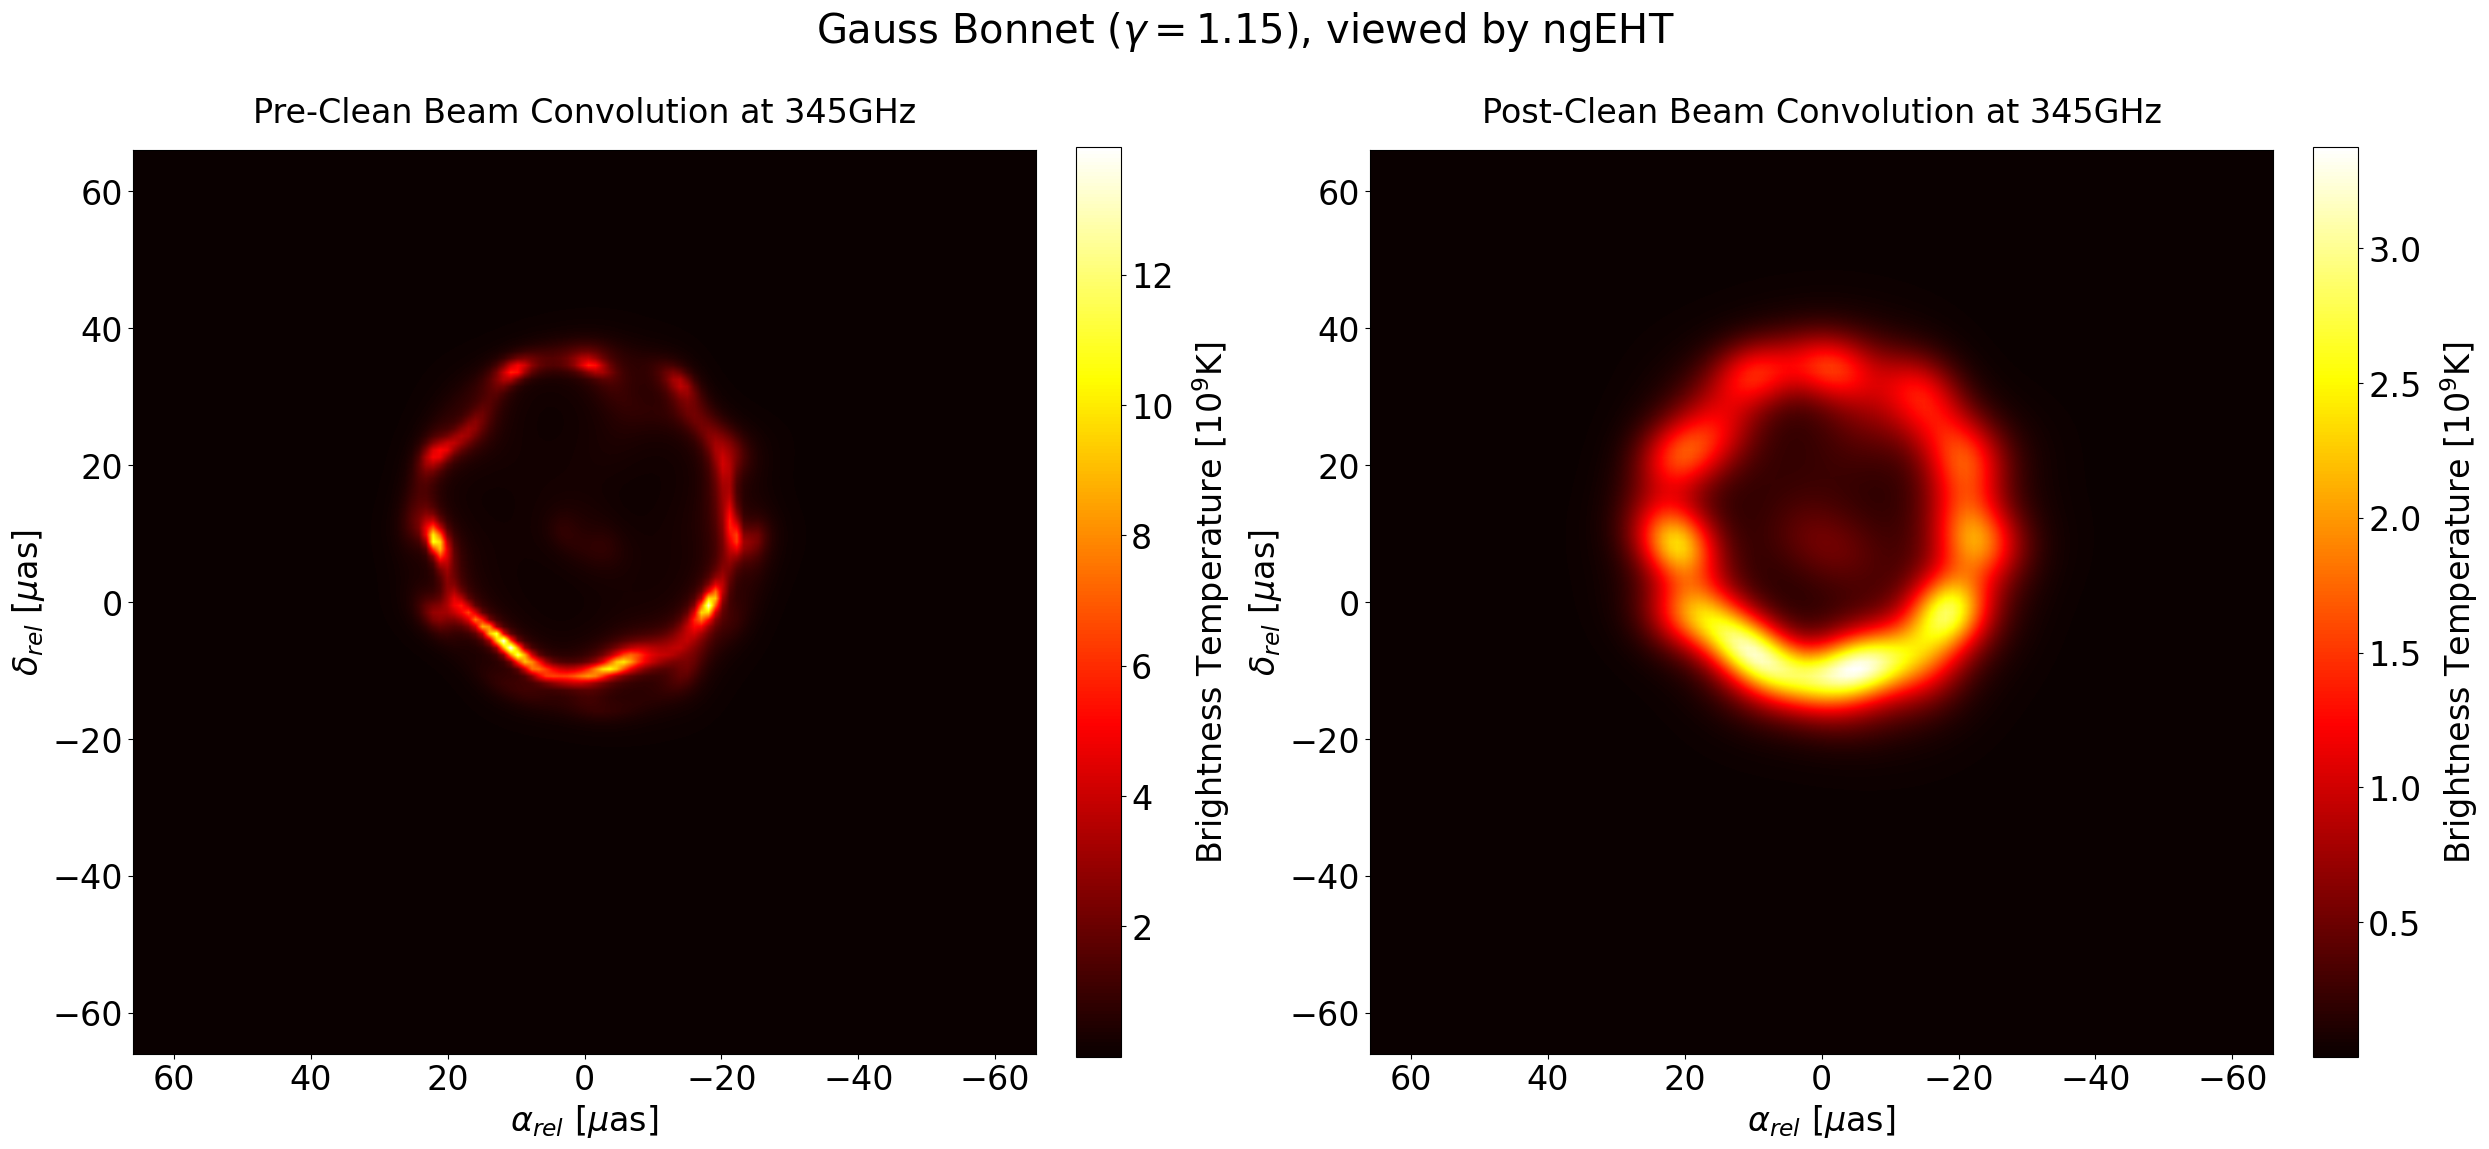
\includegraphics[scale = 0.23]{Ehtim_plot_ngEHT_no_blur_345_GB.png}
	\end{subfigure}\\
	\label{Naked_Singularity_EHT_ng2017}
	\caption[Реконструирани образи на голи сингулярности, при избрани стойности на $\gamma$, от ngEHT]{\small Реконструирани образи на голи сингулярности, при избрани стойности на $\gamma$, от ngEHT. Левият панел показва "голата"$\,$ реконструкция, преди коволюцията с "чистия сноп". Финалните стойности на $\chi^2$ са $\chi^2_\text{amp} = \{1.00, 0.99\}$ и $\chi^2_\text{cl. phase} = \{1.53, 1.46\}$, съответно за Гаус-Боне и Джанис-Нюман-Уиникър.} 
\end{figure}

\subsection{Темплейтен анализ}

За да направим количествено описание на реконструкциите, трябва да въведем величини, характеризиращи геометрията им. Колаборацията EHT въведоха за целта темплейт на пръстен с Гаусова дебелина, който фитираха към изображенията си \cite{EHT_M87_VI}. Той се характеризита с диаметър, дебелина и ориентация. Фитираните стойности на тези параметри се приемат за геометричните характеристики на реконструкциите. Ние ще подходим по подобен начин, възползвайки се от софтуерният пакет VIDA$^{20}$ \cite{VIDA}. Той приема за "вход"$\,$ реконструиран образ, към който фитира избран от нас темплейт, извършвайки многомерна минимизация. Избираме да работим с елипсовиден темплейт, с Гсаусова дебелина, описван от следните параметри: централна позиция $(x_0,y_0)$, диаметър $d$ и елиптичност $\tau$, свързани с двете пулооси посредством $d = 2\sqrt{ab}$, $\tau = 1 - b/a$, дебелина $\mathcal{\omega} = 2\sqrt{2\ln2}\sigma$ и ъгъла на ориентация на голямата пулоос $\xi_\tau$. За да отчетем асиметрията на реконструкциите, предизвикана от ефекта на Доплер, към темплейта добавяме и излъчваща арка, дефинирана като:
\begin{equation}
	S(x,y;s,\xi_s) = N_0(1 + s\cos(\phi - \xi_s)),
\end{equation}
където $s$ е относителният интензитет на арката и $\xi_s$ е ъгълът ѝ на ориентацията. Параметърът $N_0$ служи за нормиране на (8.10) към единица. С това можем да запишем израз за пълният темплейт:
\begin{equation}
	h(x,y) = S(x,y;s,\xi_s)e^{-\frac{(d(x,y))^2}{2\sigma^2}}\in[0,1],
\end{equation}
където $d(x,y)$ е минималното разстояние между точката с координати $(x,y)$, и елипсата с параметри $\{d_0,\tau,x_0,y_0\}$. Темплейтът, най-добре описващ дадена реконструкция приемаме за този, който минимизира \emph{дивергенцията на Батачаря} \footnote{Тази величина е първоначално въведена като мярка за приликата между две вероятностни разпределения - $Bh(a(x),b(x)) = 0$ означава, че $a(x) = b(x)$, докато $Bh(a(x), b(x)) = \infty$, че $a(x)$ и $b(x)$ са "ортогонални"$\,$ в смисъл, че сечението на двете разпределения е нулево.}:
\begin{equation}
	Bh\left(I(x,y)||h(x,y)\right)= -\log\int\sqrt{I(x,y)h(x,y)}dxdy,
\end{equation}
която сравнява темплейта $h(x,y)$, с изображението $I(x,y)$.\\

Имайки параметрите на темплейта, можем по систематичен начин да дефинираме границите на излъчващият пръстен. Следвайки \cite{Eichhorn2022}, го дефинираме като регионът $\mathcal{R}$:

\begin{equation}
	\mathcal{R}=\left\lbrace
	(x,y)\in\mathbb{R}^2\;:\;d(x,y;\,r_0,\tau,\xi_\tau,x_0,y_0)\leqslant\sigma\right\rbrace\;,
\end{equation}

докато централната депресия $\mathcal{S}$ дефинираме като:

\begin{equation}
	\mathcal{S} = \left\lbrace (x,y)\in\mathbb{R}^2: \sqrt{x^2 + y^2} < d(x,y;r_0,\tau,\xi_\tau,x_0,y_0) - \sigma\right\rbrace
\end{equation}

Сега можем да въвеждам количествената мярка за морфологията на централната депресия $\hat{f}_c$:
\begin{equation}
	\hat{f}_c = \frac{\text{минималният поток в }\mathcal{S}}{\text{средният поток в }\mathcal{R}}.
\end{equation}

\subsubsection{Темплейтен анализ на реконструкциите от EHT 2017}

Фитираните темплейти, заедно със самите реконструкции, са показани на фигура 8.6. Показваме също хоризонталните и вертикалните сечения през центъра и на двата образа. Параметрите на темплейтите са обобщени в таблица \ref{table:VIDA_2017}\\

Виждаме, че свойствата на реконструираният образ на голата сингулярност на Гаус-Боне, са сходни с тези на черни дупки на Кер. Още повече - те са в съгласие с параметрите, получени от екипа на EHT при анализът им на M87$^*$ \cite{EHT_M87_VI}. Следователно голи сингулярности на Гаус-Боне могат да доведат до наблюдавани образи, напълно съвместими с тези на M87$^*$.\\

\begin{table}[h!]
	\centering
	\begin{tabular}{c|c|c|c|c}
		\hline
		{Параметър на темплейта} & {Шварцшилд}&{Кер (a=0.5)}&{Гаус-Боне}&{Д.Н.У.}
		\\\hline\hline
		$\sigma$ {(\small дебелина на пръстена [$\mu$as])} & 6.17&6.21&7.26&7.94
		\\
		$\tau$ {(\small елиптичност)} & 0.10&0.10&0.18&0.15
		\\
		$\xi_\tau$ {(\small ориентация на елипсата)} & -1.95&1.19&-1.96&-1.95
		\\
		$s$ {(\small отн. интензитет на арката)} & 0.28 &0.34 & 0.29 & 0.17
		\\
		$\xi_s$ {(\small ориентация на арката)} & -1.78 &-1.85 &-1.73 & -1.77
		\\\hline
		$r_0$ {(\small радиус на пръстена [$\mu$as])} & 21.1 &21.1&21.0 & 15.4
		\\
		$x_0$ {(\small отместване по RA [$\mu$as])} & -8.78 &-9.47&-11.37 & 1.38
		\\
		$y_0$ {(\small отместване по DEC [$\mu$as])} & 9.61 & 9.46&12.68&-4.10
		\\\hline\hline
		{Оптимизирана дивергенция} & 0.005 & 0.006&  0.007 & 0.004
		\\ \hline
	\end{tabular}
	\caption[Параметри на темплейтния анализ за EHT 2017.]{\small Параметри на темплейтния анализ за EHT 2017. За сравнение, извършваме анализа и за двете черни дупки на Кер при параметри на въртене $a =\{0,0.5\}$.}
	\label{table:VIDA_2017}
\end{table}

От друга страна, голата сингулярност на Джанис-Нюман-Уиникър води до значително по-малък диаметър на образа. Той зависи силно от свойствата на излъчващата среда, като в нашият случай, се влияе от стойността на $r_0$. Освен това обаче, се влияе силно и от геометрията на пространство-времето, чрез ефекта на гравитационната леща. Вече е показано, че слаби сингулярности на Джанис-Нюман-Уиникър, със скаларен параметър $\gamma <0.53$, водят до диаметри на техните образи, които не са съвместими с наблюденията на М87$^*$. Това може да се обясни чрез по-силният фокусиращ ефект на пространство-времето с намаляването на $\gamma$. Същият аргумент може да се приложи и за нашият случай на силна сингулярност $\gamma = 0.48$. Чрез напасване на параметъра $r_0$, ние \emph{не} успяхме да възпроизведем диаметър на образа, който да е в съгласие с този на M87$^*$. Следователно можем да заключим, че в този случай, по-малкият видим диаметър на образа е свойство на самото пространство-време, а не толкова на спецификите на модела на излъчващата среда.\\

От друга страна виждаме, че централната депресия при двете екзотични решения показва значително по-висок поток от черните дупки на Кер. Това е отразено и в таблица \ref{table:f_2017}, където са показани стойностите на количествената мярка $\hat{f}_c$.

\begin{table}[h!]
	\centering
	\begin{tabular}{||c|c|c|c|c||}
		\hline
		{Метрика} & {Шварцшилд}&{Кер (a=0.5)}&{Гаус-Боне}&{Д.Н.У.}
		\\\hline
		{\thead{$\hat{f}_c$}} & 0.026&0.030&0.239&0.451
		\\\hline
	\end{tabular}
	\caption[Количествената мярка $\hat{f}_c$ за морфологията на централата депресия на EHT 2017]{\small Количествената мярка $\hat{f}_c$ за морфологията на централата депресия на EHT 2017, за разглежданите метрики. За сравнение сме пресметнали $\hat{f}_c$ и за черните дупки на Кер.}
	\label{table:f_2017}
\end{table}

Виждаме, че параметърът на въртене не променя значително стойността на $\hat{f}_c$ за черни дупки на Кер. Той остава съразмерим с получените от EHT резултати (използвайки различен темплейт) $\hat{f}_c(\text{M}87^*) = 0.04$ \cite{EHT_M87_IV}. Също така виждаме, че $\hat{f}_c$ за голите сингулярности са с един порядък по-високи. Това показва, че дори да не можем да разделим оптически централните пръстени, реконструкцията все пак е чувствителна към тях, и те оставят "отпечатък"$\,$ в крайният образ\footnote{Тук трябва да се внимава обаче, понеже тази количествена мярка е силно чувствителна към метода за реконструкция. Ако го използваме за съдене на наличието на екзотични образи, би следвало да изискваме той да е с поне \emph{два} порядъка по-висок от този за черни дупки.}.

\newpage

\begin{figure}[h!]
	\centering
	\begin{subfigure}{12cm}
		\hspace{-1.5cm}
		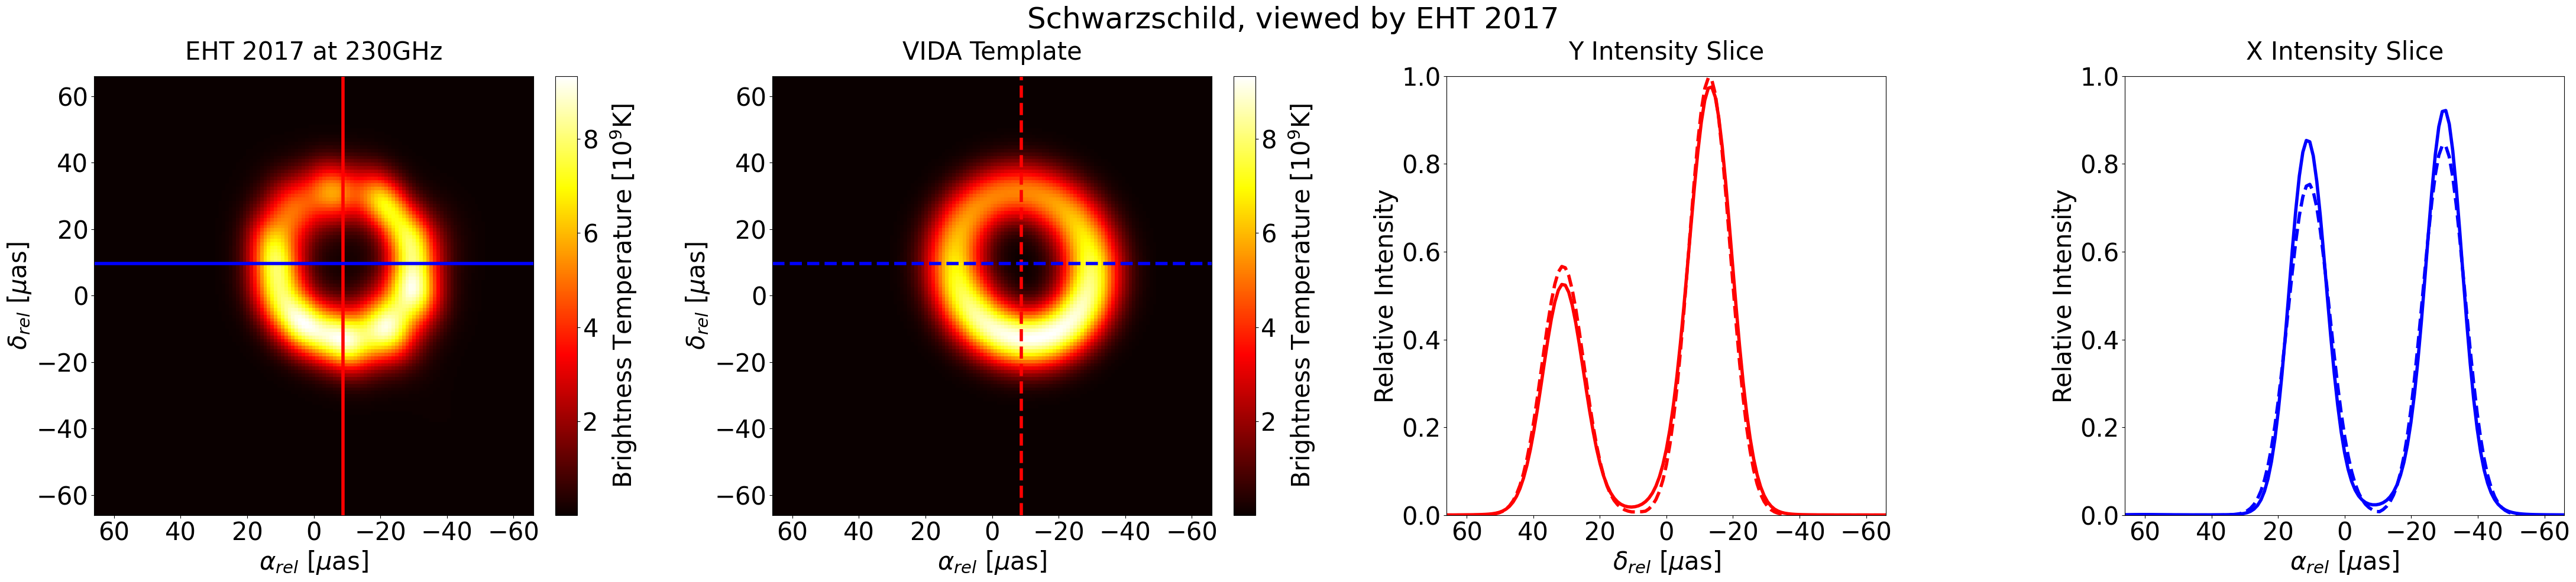
\includegraphics[scale = 0.13]{Ehtim_Vida_plot_2017_230_Sch.png}
	\end{subfigure}\\
		\begin{subfigure}{12cm}
		\hspace{-1.5cm}
		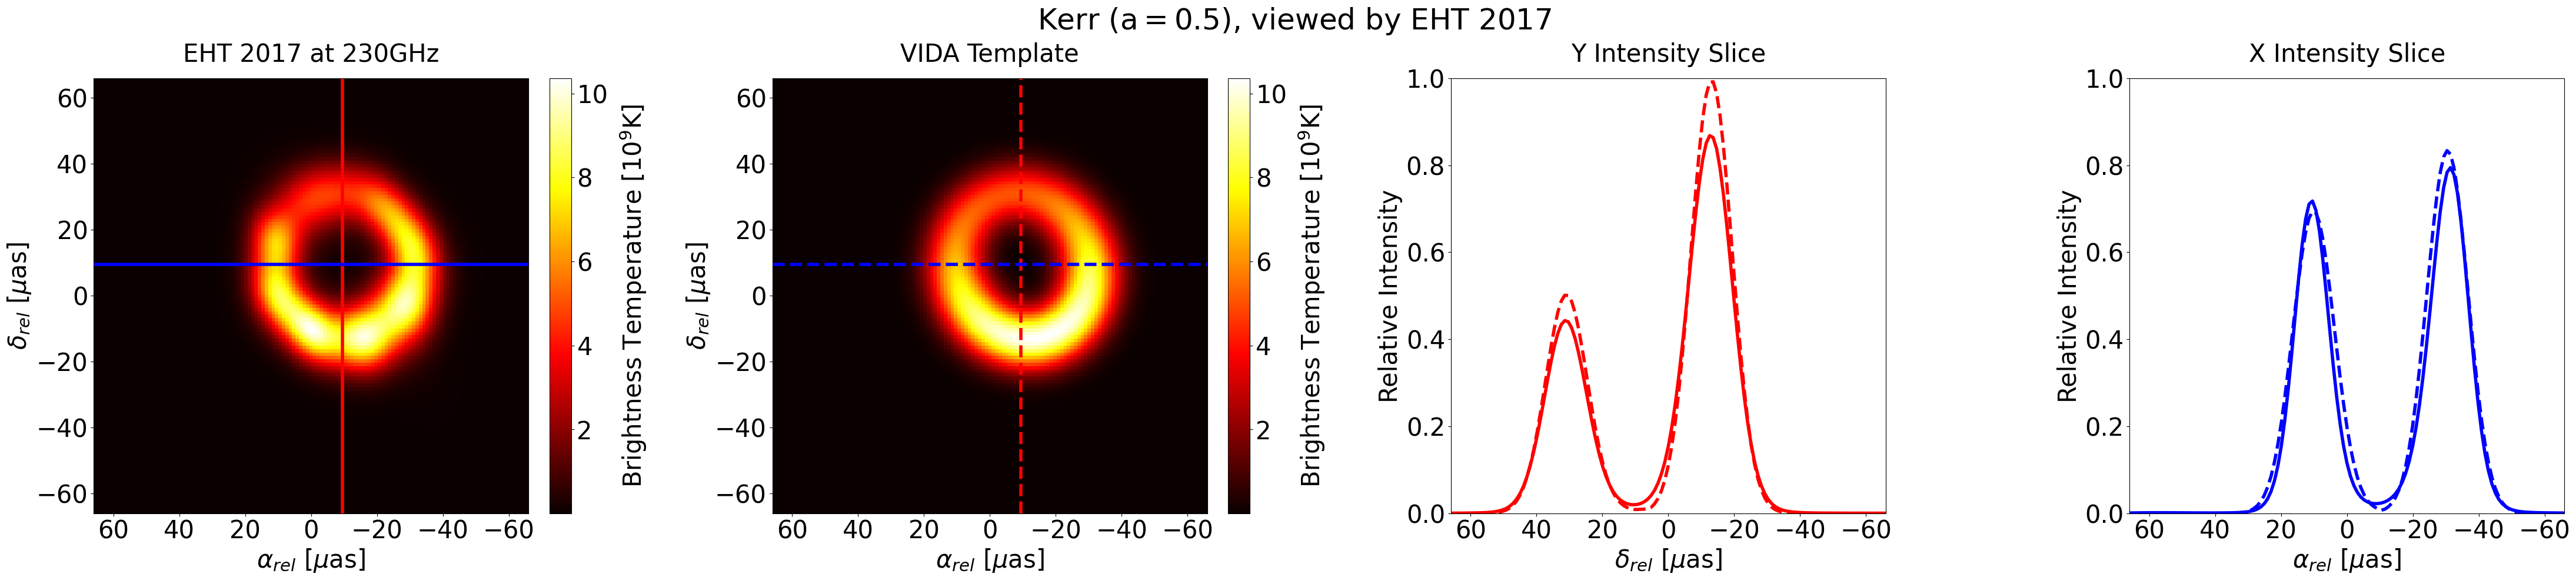
\includegraphics[scale = 0.13]{Ehtim_Vida_plot_2017_230_Kerr.png}
	\end{subfigure}\\
	\begin{subfigure}{12cm}
		\hspace{-1.5cm}
		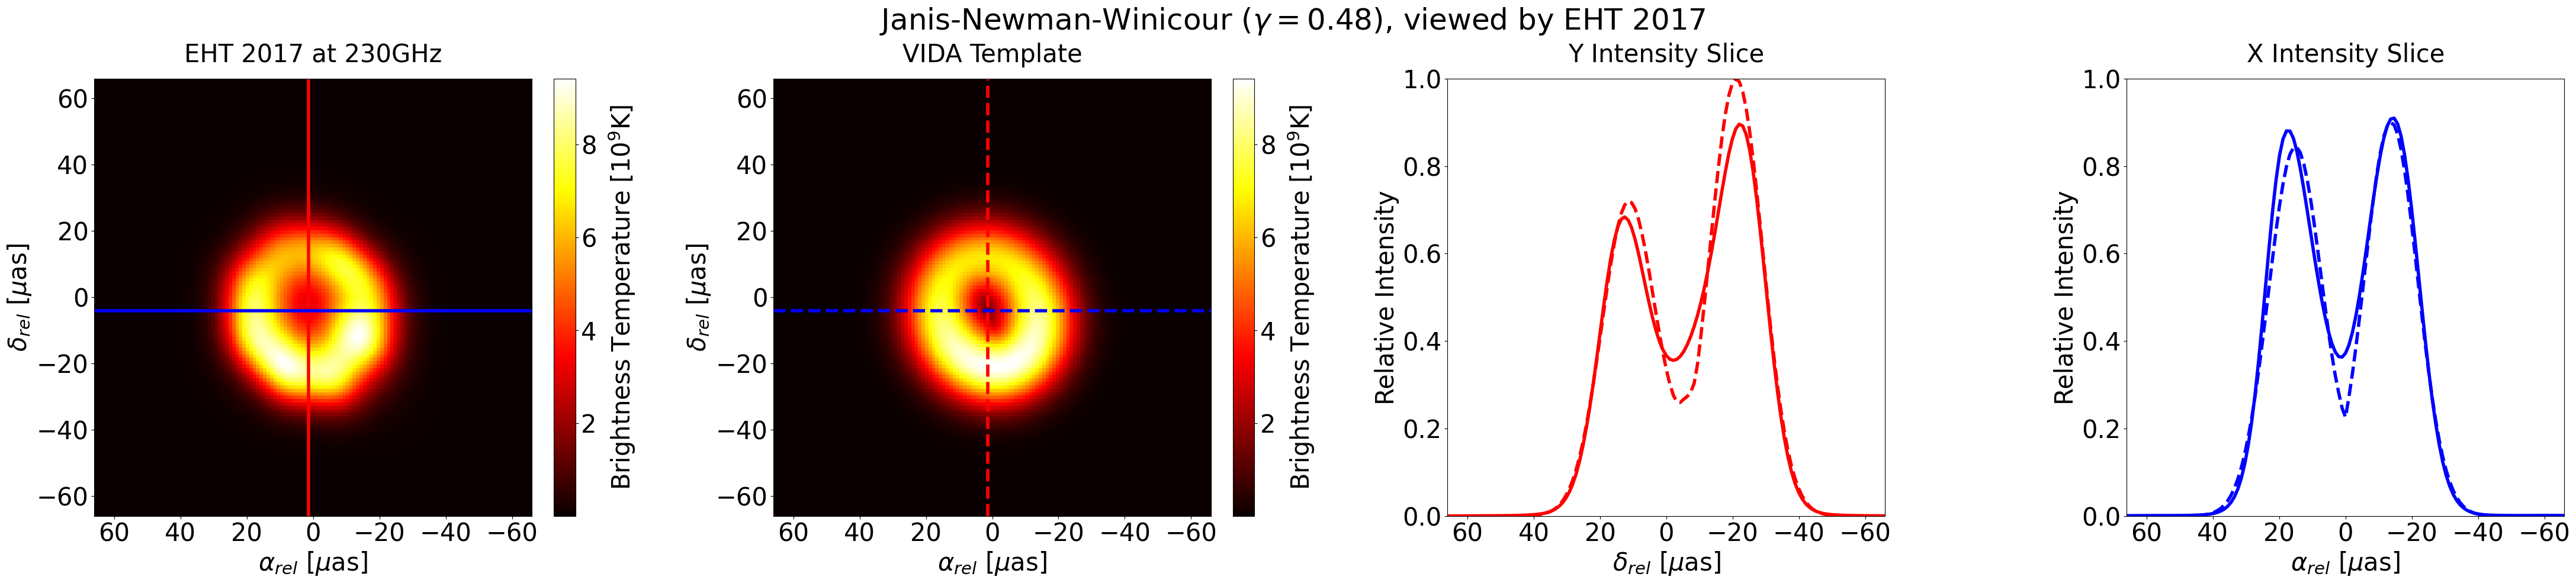
\includegraphics[scale = 0.13]{Ehtim_Vida_plot_2017_230_JNW.png}
	\end{subfigure}\\
	\begin{subfigure}{12cm}
		\hspace{-1.5cm}
		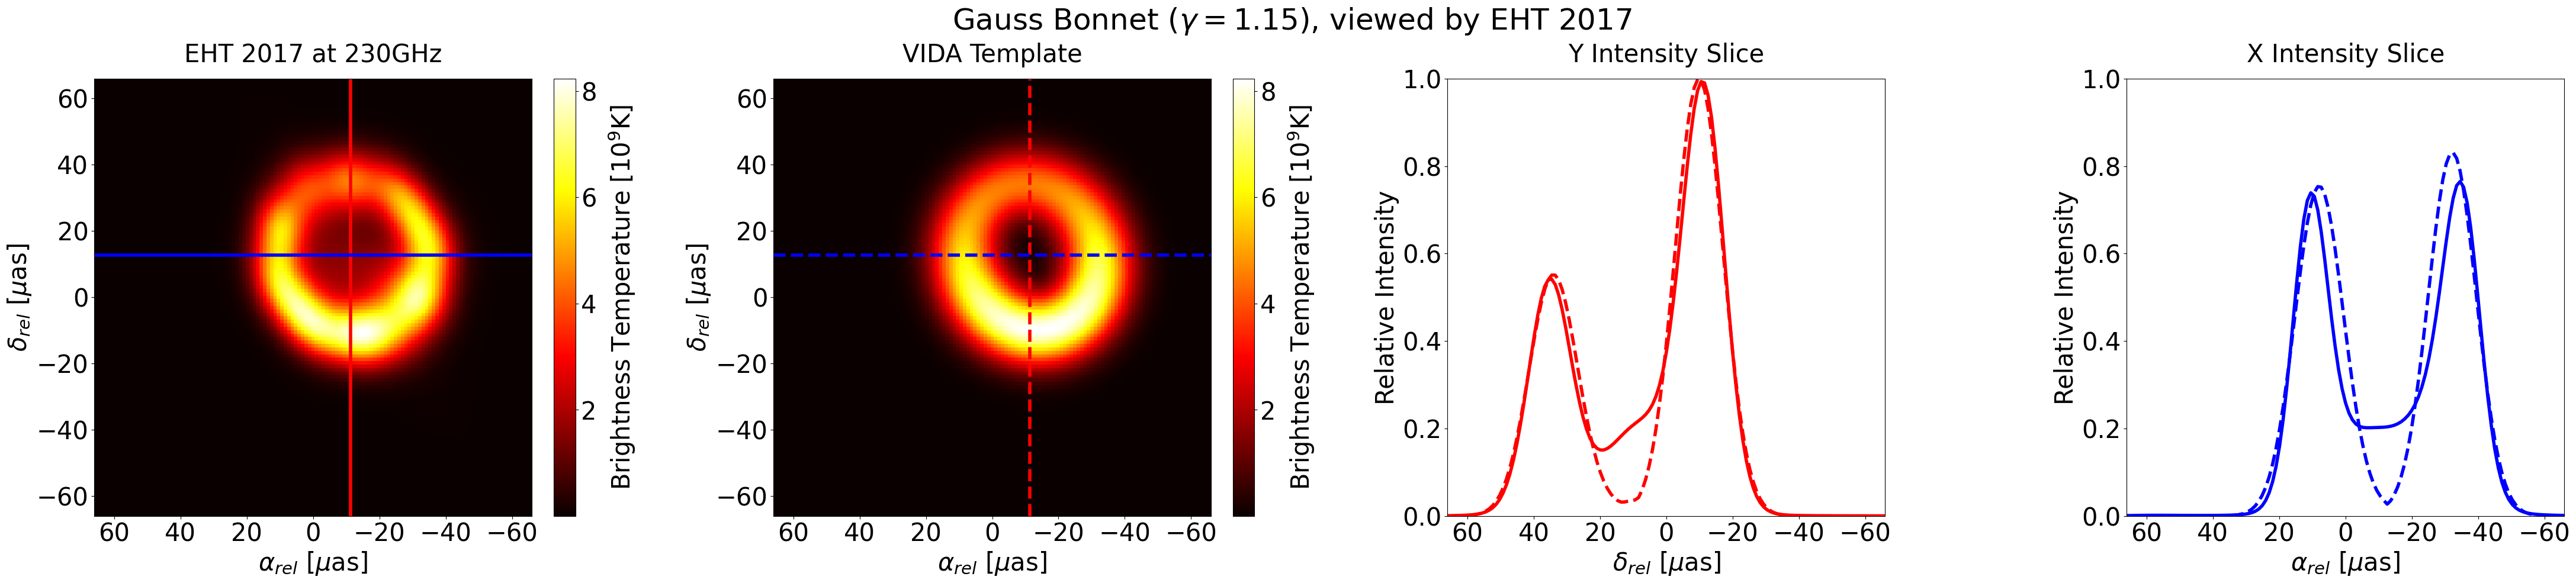
\includegraphics[scale = 0.13]{Ehtim_Vida_plot_2017_230_GB.png}
	\end{subfigure}\\
	\label{VIDA_EHT_ng2017}
	\caption[Темплейтен анализ на реконструкциите от EHT 2017]{\small Темплейтен анализ на реконструкциите от EHT 2017. На десните два панела показваме профила на интензитета, и за двата образа, през центъра $(x_0,y_0)$ на темплейта.} 
\end{figure}

\subsubsection{Темплейтен анализ на реконструкциите от EHT 2022}

В таблица \ref{table:f_2022} представяме количествената мярка $\hat{f}_c$ за разширената конфигурация на телескопи EHT 2022, докато в таблица \ref{table:VIDA_2022} представяме параметрите на темплейтите.

\begin{table}[h!]
	\centering
	\begin{tabular}{||c|c|c|c|c||}
		\hline
		{Метрика} & {Шварцшилд}&{Кер (a=0.5)}&{Гаус-Боне}&{Д.Н.У.}
		\\\hline
		{\thead{$\hat{f}_c$}} & 0.009&0.009&0.180&0.290
		\\\hline
	\end{tabular}
	\caption[Количествената мярка $\hat{f}_c$ за морфологията на централата депресия на EHT 2022]{\small Количествената мярка $\hat{f}_c$ за морфологията на централата депресия на EHT 2022, за разглежданите метрики.}
	\label{table:f_2022}
\end{table}
Виждаме, че повишената резолюция намалява видимото "размиване"$\,$на лъчението в централната депресия, в следствие на което $\hat{f}_c$ намалява за всички реконструкции. Това намаляване обаче е по-малко за голите сингулярности. 
\begin{figure}[h!]
	\centering
	\begin{subfigure}{12cm}
		\hspace{-1.5cm}
		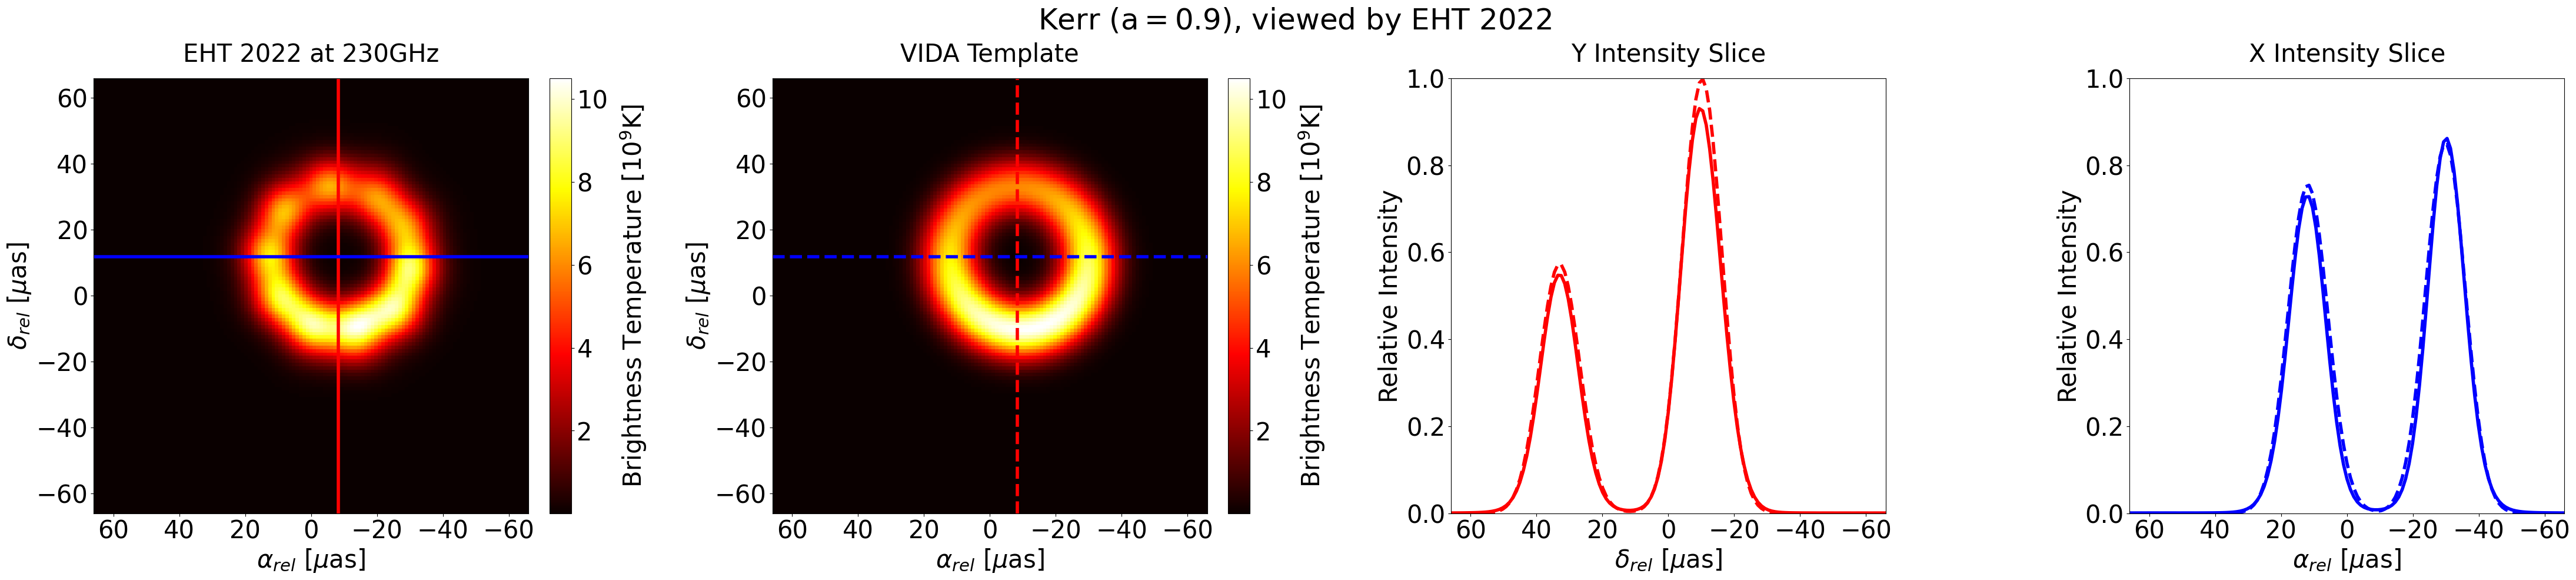
\includegraphics[scale = 0.13]{Ehtim_Vida_plot_2022_230_Sch.png}
	\end{subfigure}\\
	\begin{subfigure}{12cm}
		\hspace{-1.5cm}
		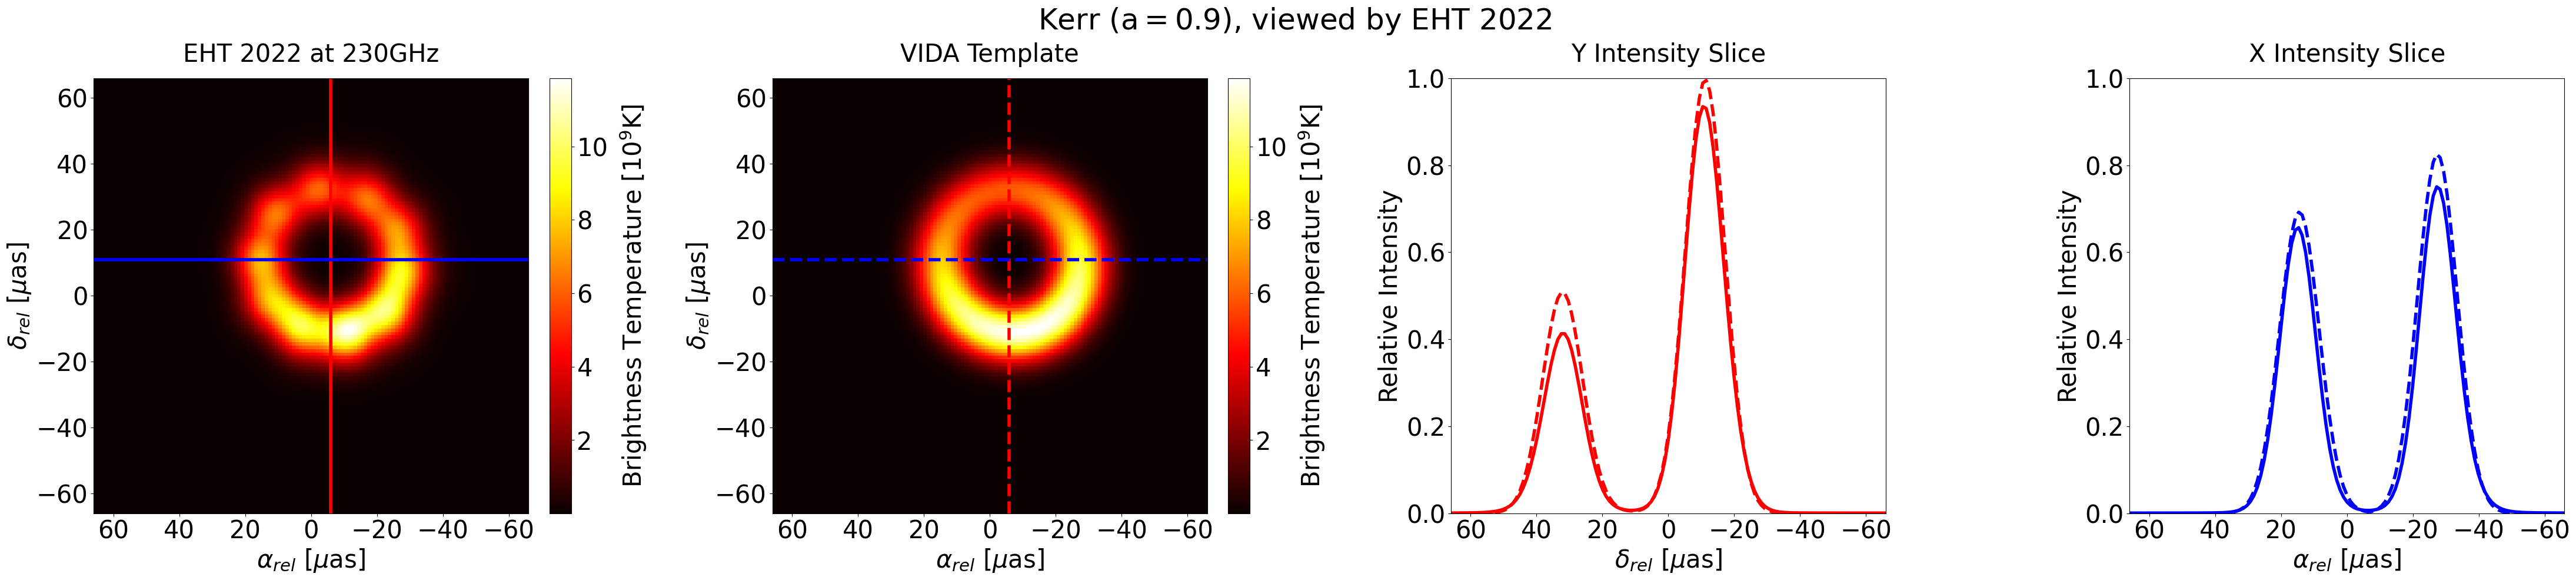
\includegraphics[scale = 0.13]{Ehtim_Vida_plot_2022_230_Kerr.png}
	\end{subfigure}\\
	\begin{subfigure}{12cm}
		\hspace{-1.5cm}
		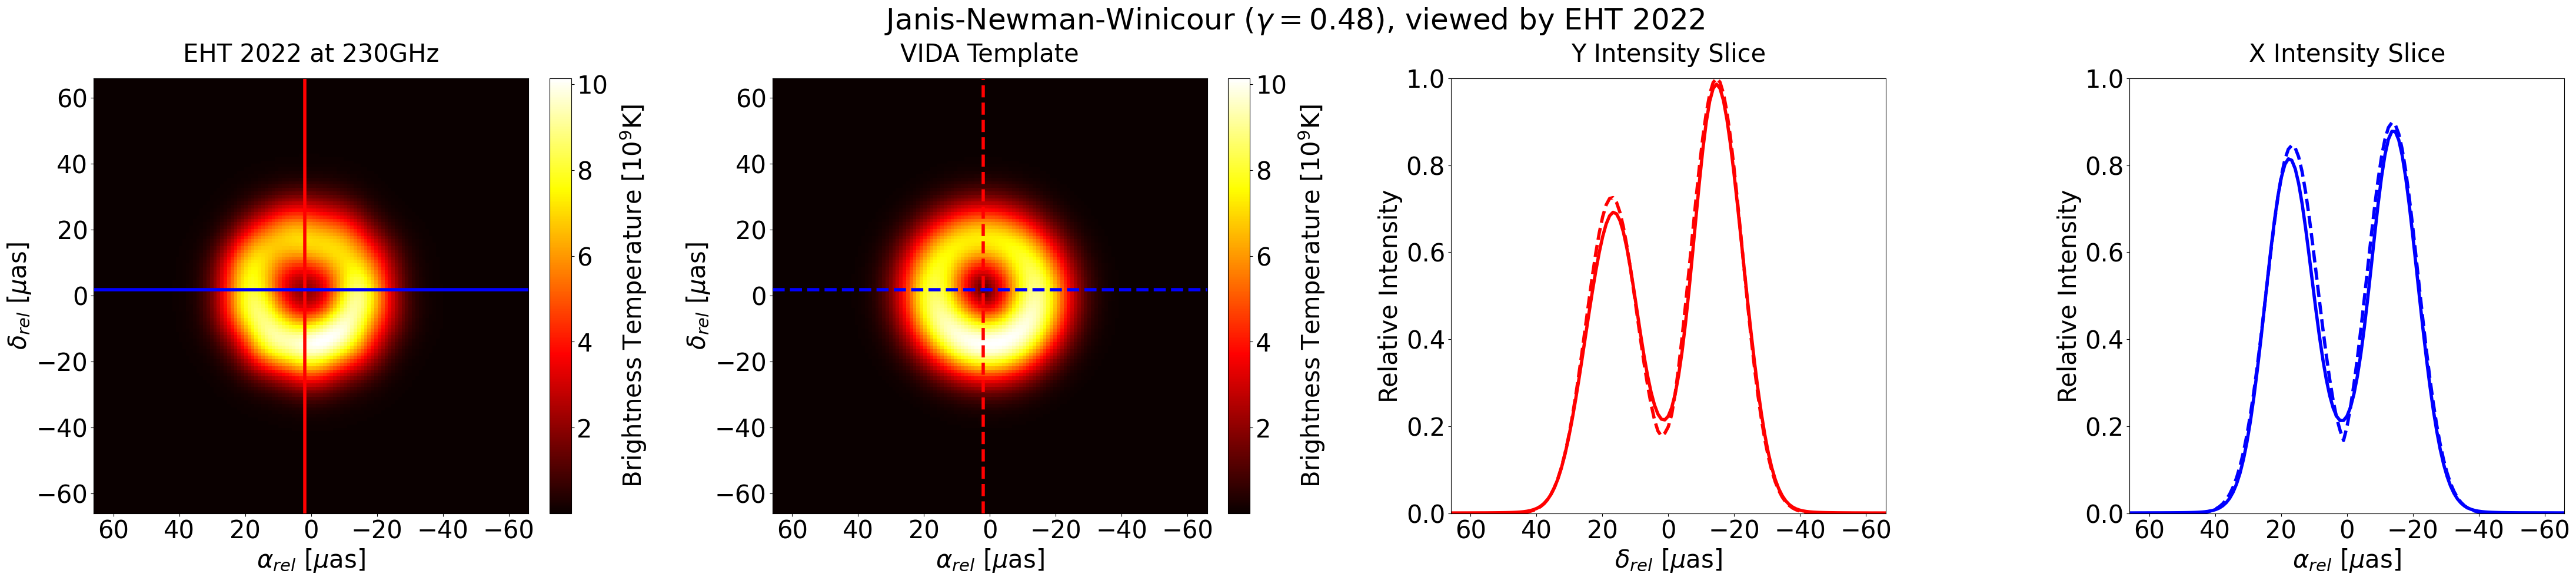
\includegraphics[scale = 0.13]{Ehtim_Vida_plot_2022_230_JNW.png}
	\end{subfigure}\\
	\begin{subfigure}{12cm}
		\hspace{-1.5cm}
		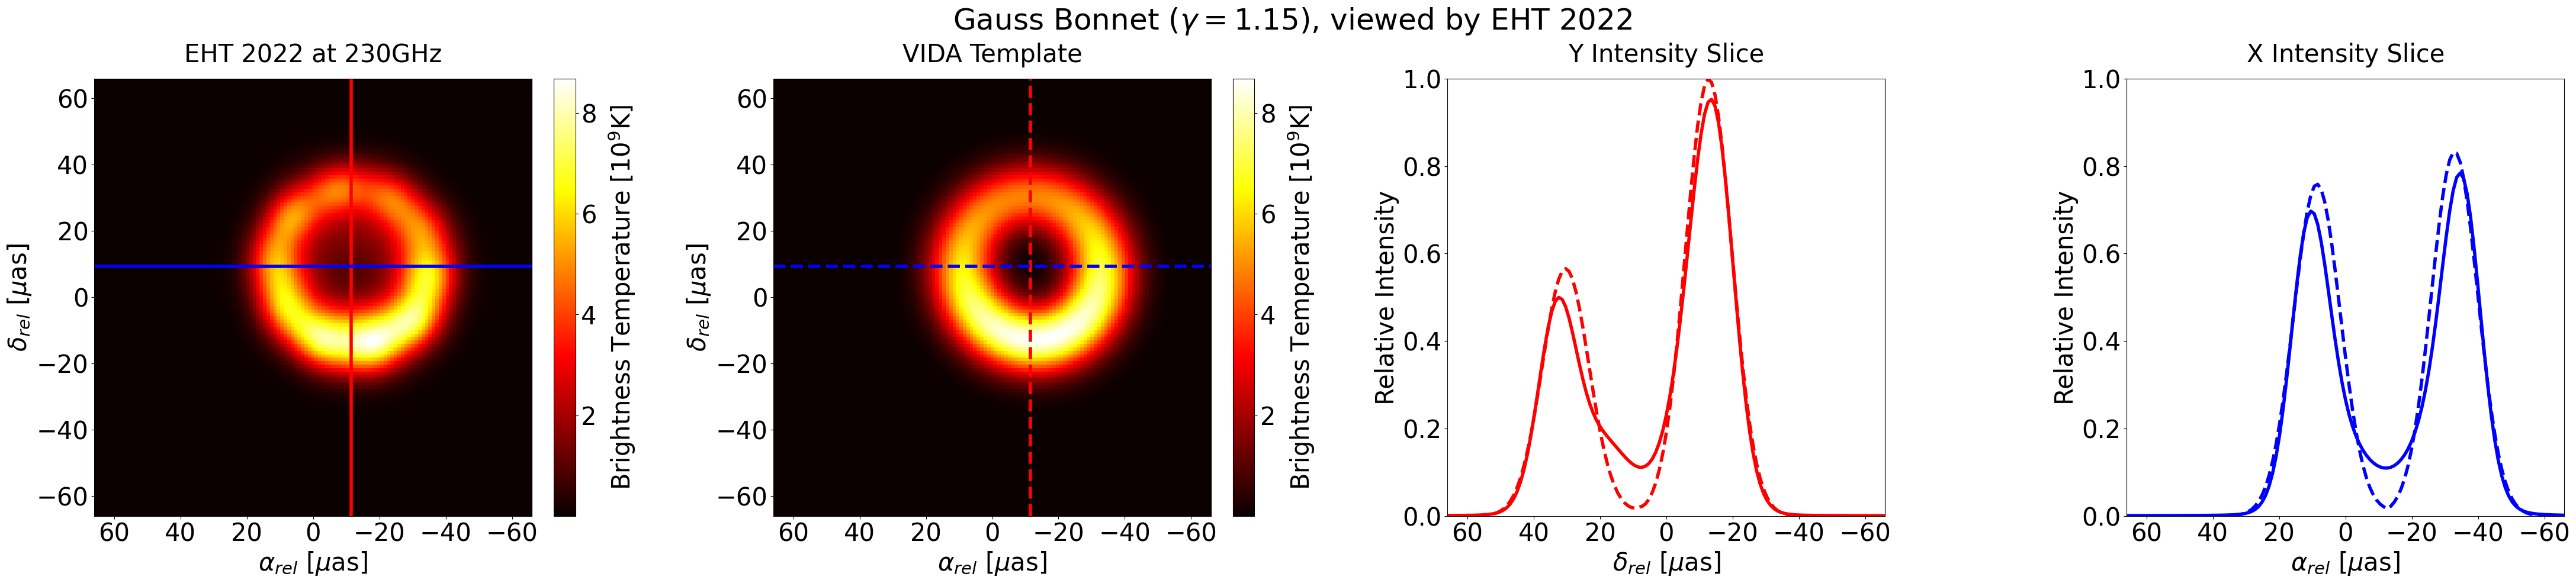
\includegraphics[scale = 0.13]{Ehtim_Vida_plot_2022_230_GB.png}
	\end{subfigure}\\
	\label{VIDA_EHT_ng2022}
	\caption[Темплейтен анализ на реконструкциите от EHT 2022]{\small Темплейтен анализ на реконструкциите от EHT 2022. На десните два панела показваме профила на интензитета, и за двата образа, през центъра $(x_0,y_0)$ на темплейта.} 
\end{figure}
\newline

\begin{table}[h!]
	\centering
	\begin{tabular}{c|c|c|c|c}
		\hline
		{Параметър на темплейта} & {Шварцшилд}&{Кер (a=0.5)}&{Гаус-Боне}&{Д.Н.У.}
		\\\hline\hline
		$\sigma$ {(\small дебелина на пръстена [$\mu$as])}& 5.97& 5.98& 6.95& 7.69
		\\
		$\tau$ {(\small елиптичност)} & 0.04& 0.04& 0.05& 0.06
		\\
		$\xi_\tau$ {(\small ориентация на елипсата)}& -1.93& 1.24& -1.95& -1.96
		\\
		$s$ {(\small отн. интензитет на арката)} & 0.28& 0.34& 0.28& 0.16
		\\
		$\xi_s$ {(\small ориентация на арката)}  & -1.79& -1.83& -1.74& -1.76
		\\\hline
		$r_0$ {(\small радиус на пръстена [$\mu$as])} & 21.2& 21.2& 21.1&15.4
		\\
		$x_0$ {(\small отместване по RA [$\mu$as])}  & -8.35& -5.89& -11.47& 1.97
		\\
		$y_0$ {(\small отместване по DEC [$\mu$as])} & 11.85& 10.94& 9.32& 1.79
		\\\hline\hline
		{Оптимизирана дивергенция} & 0.002& 0.003& 0.004& 0.002
		\\ \hline
	\end{tabular}
	\caption[Параметри на темплейтния анализ за EHT 2022.]{\small Параметри на темплейтния анализ за EHT 2022. За сравнение, извършваме анализа и за двете черни дупки на Кер при параметри на въртене $a =\{0,0.5\}$.}
	\label{table:VIDA_2022}
\end{table}

\newpage

Следователно разликата между тях и черните дупки е по-ясно изразена тук - отношението между техните $\hat{f}_c$ мерки нараства приблизително 2 пъти. 
На фигура 8.8 е показан самия темплейтен анализ. Можем да забележим, че има много по-добро съгласие в сеченията през $(x_0,y_0)$ между реконструкцията и темплейта.


\subsubsection{Темплейтен анализ на реконструкциите от ngEHT}

Както видяхме от фигура 8.6, наблюденията на ngEHT при 345 GHz стават чувствителни към централните образи и реконструкциите добиват ясен локален максимум в централната депресия. Използваме фитираните темплейти (таблици \ref{table:VIDA_ngEHT} и \ref{table:VIDA_ngEHT_1}) за изолираме тази депресия и да анализираме морфологията на максимумите. На фигура 8.9 сме начертали изоконтурите на потока в центъра на образа за четирите реконструкции. Сравнили сме наблюденията при двете честоти $\nu = \{230, 345\}$ GHz, и също сме съставили тяхната суперпозиция (левите панели). Наблюдаваме, че при 345 GHz, централните максимуми достигат приблизително $15\%$ от максималният поток на образа за решението на Гаус-Боне, и $\approx 30\%$ за това на Джанис-Нюман-Уиникър. Можем също да видим, че имаме отново нарастване на отношенията на $\hat{f}_c$ между голите сингулярности и черните дупки на Кер. Като при 345 GHz то нараства приблизително 3 пъти спрямо това за EHT 2022 (таблица \ref{table:f_ngEHT}).\\

С това показваме, че централните образи наистина стават \emph{силно} наблюдателно релевантни, особено при по-високата честота 345 GHz. 

\begin{figure}[h!]
	\centering
	\begin{subfigure}{12cm}
		\hspace{-1.5cm}
		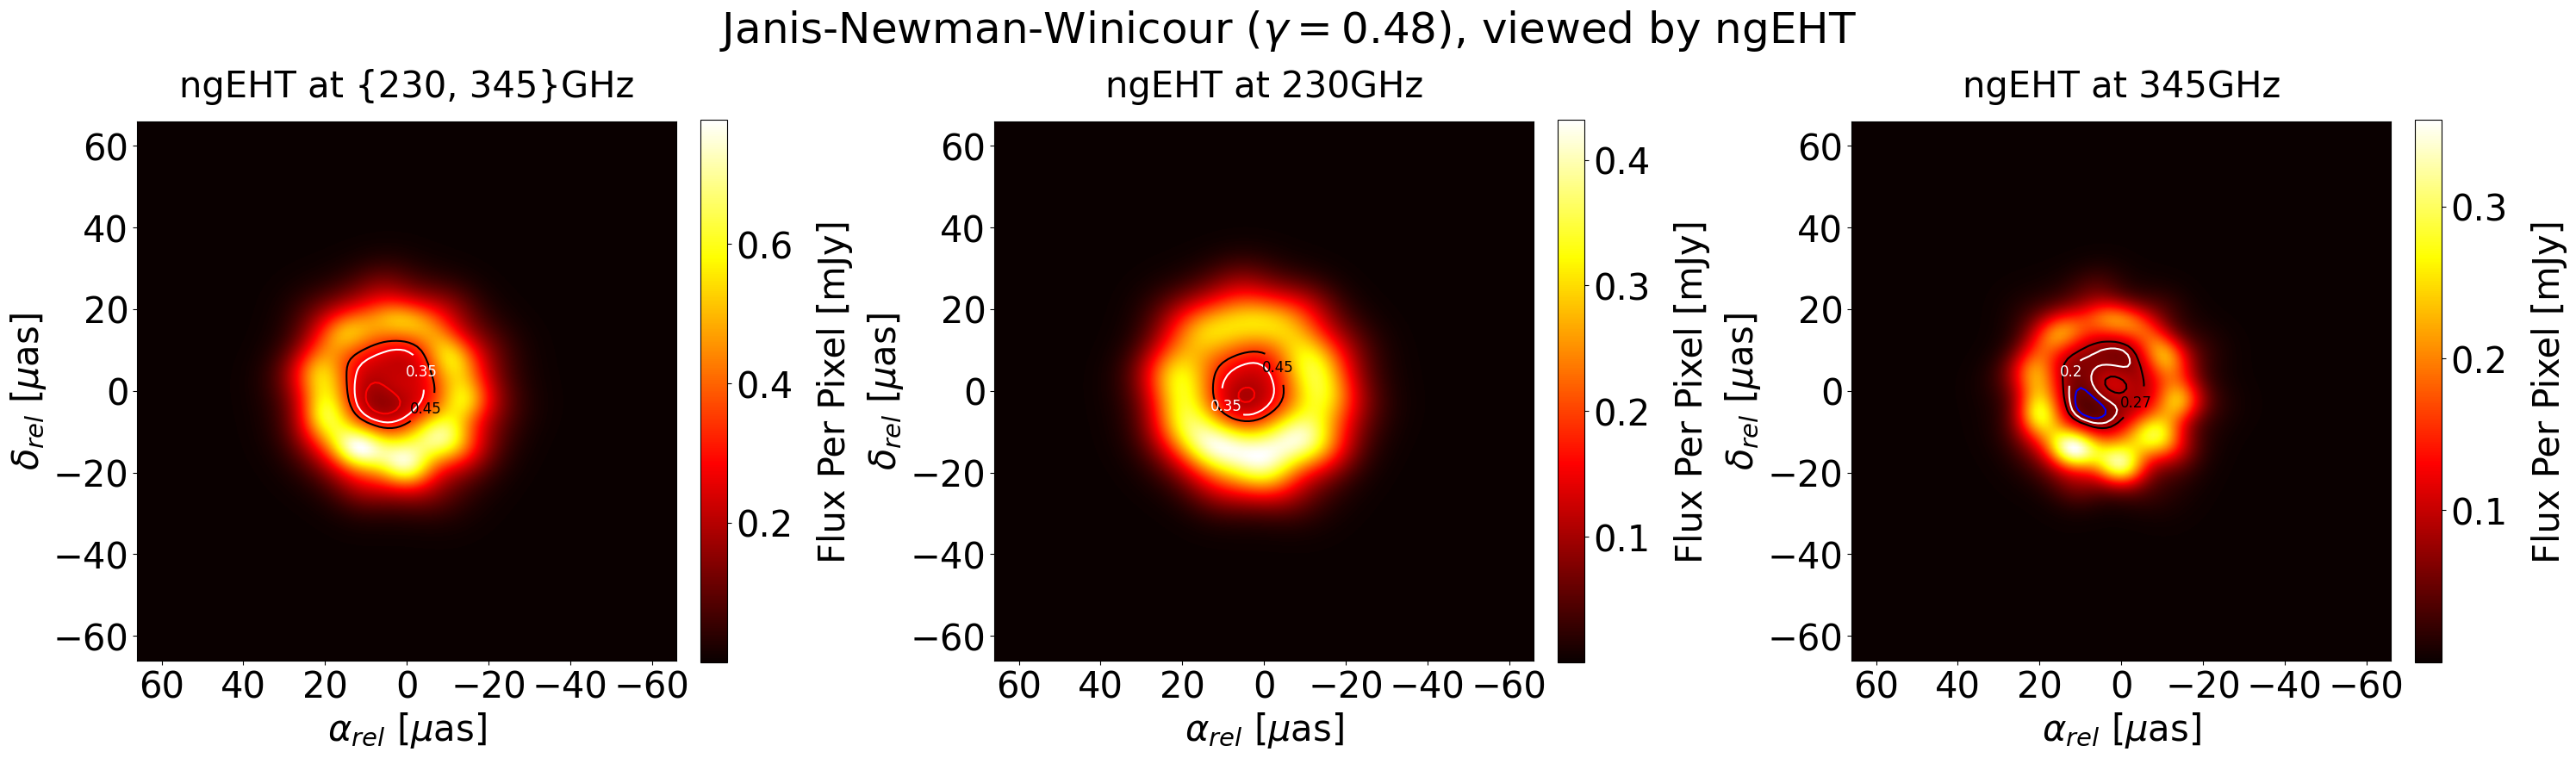
\includegraphics[scale = 0.2]{Superpos_Compare_JNW.png}
	\end{subfigure}\\
	\begin{subfigure}{12cm}
		\hspace{-1.5cm}
		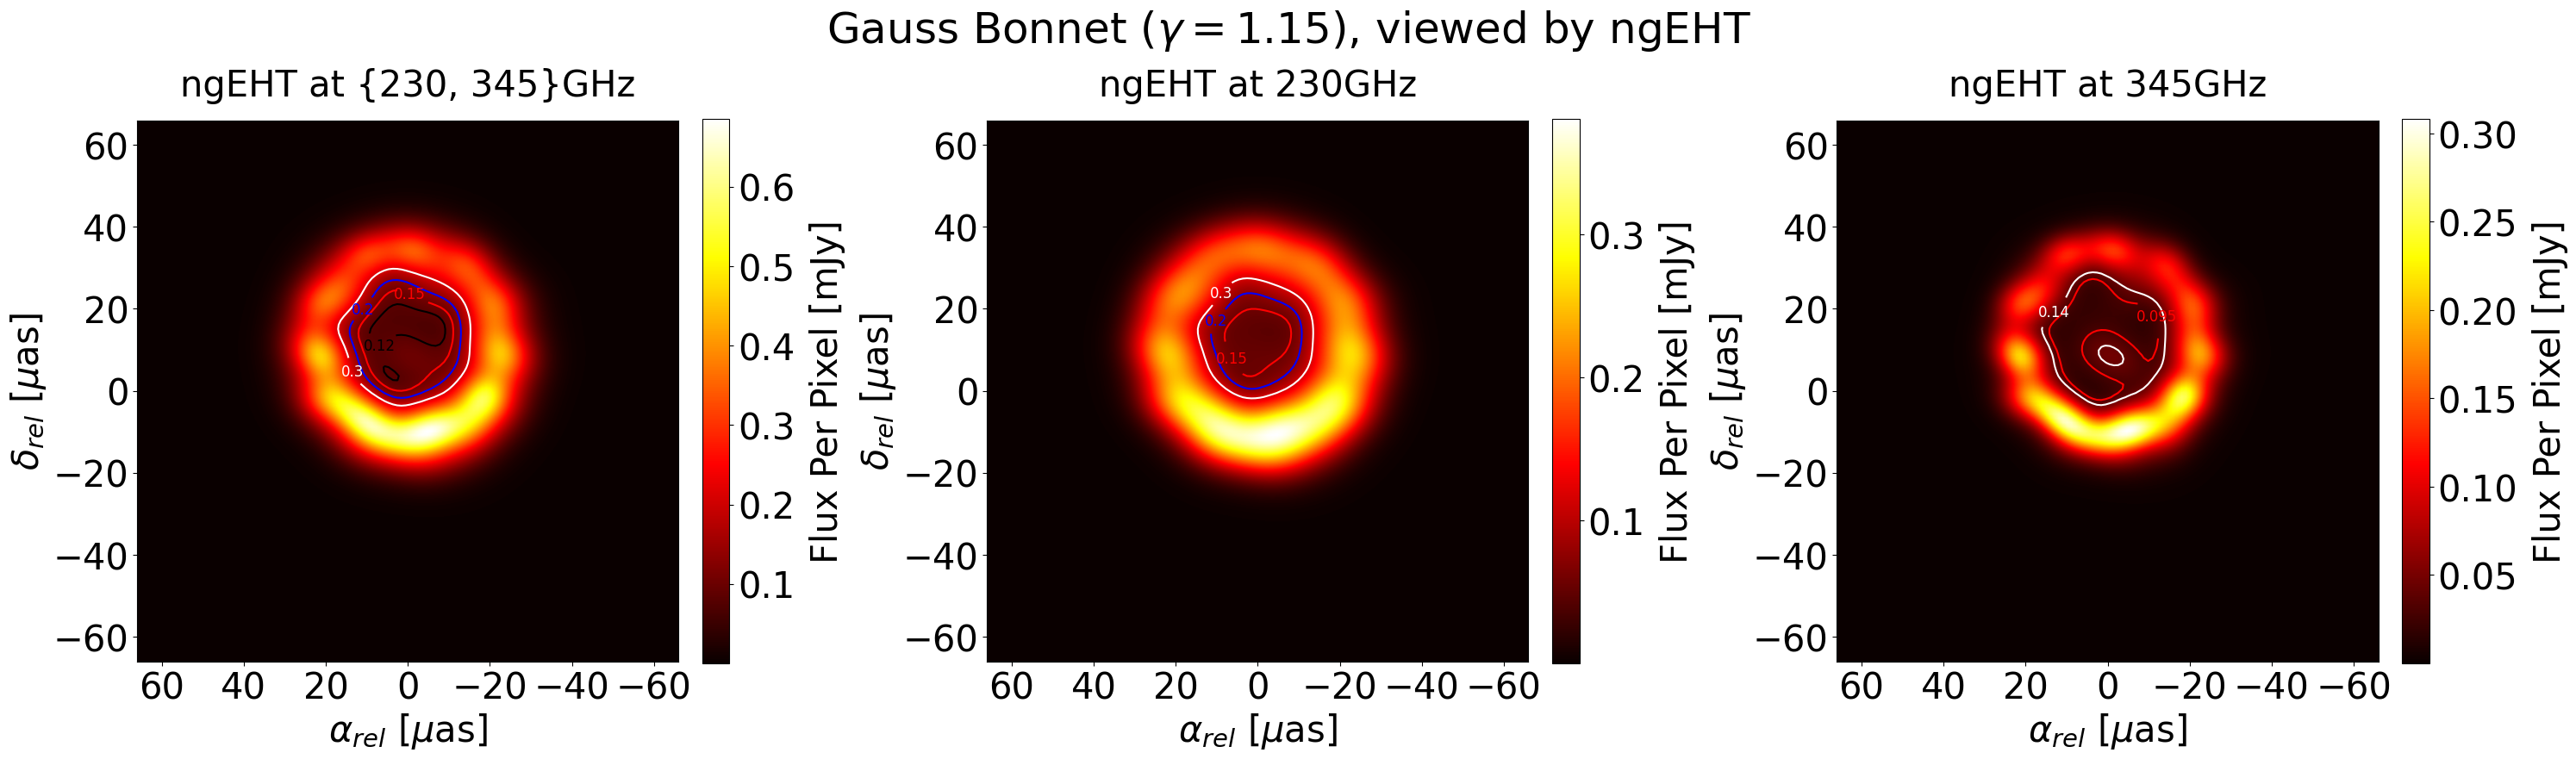
\includegraphics[scale = 0.2]{Superpos_Compare_GB.png}
	\end{subfigure}\\
	\label{isoflux_ngEHT}
	\caption[Изоконтури на потока на реконструкциите на голи сингулярности от ngEHT.]{\small Изоконтури на потока на реконструкциите на голи сингулярности от ngEHT. Обозначенията на изоконтурите са относителният поток, нормиран на максимума за съответният образ.} 
\end{figure}

\newpage

\begin{table}[h!]
	\centering
	\begin{tabular}{c|c|c|c|c}
		\hline
		{Параметър на темплейта} & {Шварцшилд}&{Кер (a=0.5)}&{Гаус-Боне}&{Д.Н.У.}
		\\\hline\hline
		$\sigma$ {(дебелина на пръстена [$\mu$as])} & 5.80&5.81&6.76&7.56
		\\
		$\tau$ {(елиптичност)} & 0.04&0.04&0.05&0.06
		\\
		$\xi_\tau$ {(ориентация на елипсата)} & -2.34&-2.30&-2.31&-2.45
		\\
		$s$ {(отн. интензитет на арката)} & 0.23&0.34&0.28&0.16
		\\
		$\xi_s$ {(ориентация на арката)} & -1.78&-1.83&-1.73&-1.78
		\\\hline
		$r_0$ {(радиус на пръстена [$\mu$as])} & 21.2&21.3&21.2&15.6
		\\
		$x_0$ {(отместване по RA [$\mu$as])} & 0.74&9.09&-0.34&3.14
		\\
		$y_0$ {(отместване по DEC [$\mu$as])} & 9.65& 14.49&10.84&0.03
		\\\hline\hline
		{Оптимизирана дивергенция} & 0.003&0.003&0.005&0.002
		\\ \hline
	\end{tabular}
	\caption[Параметри на темплейтния анализ за ngEHT, при наблюдателна честота $\nu = 230$ GHz.]{\small Параметри на темплейтния анализ за ngEHT, при наблюдателна честота $\nu = 230$ GHz.}
	\label{table:VIDA_ngEHT}
\end{table}

\begin{table}[h!]
	\centering
	\begin{tabular}{c|c|c|c|c}
		\hline
		{Параметър на темплейта} & {Шварцшилд}&{Кер (a=0.5)}&{Гаус-Боне}&{Д.Н.У.}
		\\\hline\hline
		$\sigma$ {(дебелина на пръстена [$\mu$as])} & 4.05&4.06&5.08&5.97
		\\
		$\tau$ {(елиптичност)} & 0.03&0.04&0.04&0.05
		\\
		$\xi_\tau$ {(ориентация на елипсата)} & -2.11&-2.12&1.00&-2.21
		\\
		$s$ {(отн. интензитет на арката)} & 0.36&0.45&0.38&0.23
		\\
		$\xi_s$ {(ориентация на арката)} & -1.74&-1.78&-1.73&-1.65
		\\\hline
		$r_0$ {(радиус на пръстена [$\mu$as])} & 21.0&21.0&21.4&15.6
		\\
		$x_0$ {(отместване по RA [$\mu$as])} & 0.89&9.30&-0.23&4.22
		\\
		$y_0$ {(отместване по DEC [$\mu$as])} & 1.00& 14.91&11.36&0.02
		\\\hline\hline
		{Оптимизирана дивергенция} & 0.009&0.009&0.018&0.010
		\\ \hline
	\end{tabular}
	\caption[Параметри на темплейтния анализ за ngEHT, при наблюдателна честота $\nu = 345$ GHz.]{\small Параметри на темплейтния анализ за ngEHT, при наблюдателна честота $\nu = 345$ GHz.}
	\label{table:VIDA_ngEHT_1}
\end{table}

\begin{table}[h!]
	\centering
	\begin{tabular}{||c|c|c|c|c||}
		\hline
		{Метрика} & {Шварцшилд}&{Кер (a=0.5)}&{Гаус-Боне}&{Д.Н.У.}
		\\\hline
		{\thead{$\hat{f}_c$ 230 GHz}} & 0.007&0.007&0.21&0.354
		\\\hline
		{\thead{$\hat{f}_c$ 345 GHz}} & 0.002&0.002&0.12&0.220
		\\\hline
		{\thead{$\hat{f}_c$ 230 GHz $\cup$ 345 GHz}} & 0.005&0.005&0.20&0.344
		\\\hline
	\end{tabular}
	\caption[Количествената мярка $\hat{f}_c$ за морфологията на централата депресия на EHT 2022]{\small Количествената мярка $\hat{f}_c$ за морфологията на централата депресия на EHT 2022, за разглежданите метрики.}
	\label{table:f_ngEHT}
\end{table}

За пълнота представяме и еквивалента на фигури 8.7 и 8.8, за ngEHT, при двете наблюдателни честоти $\nu = \{230, 345\}$ GHz, на фигури 8.10 и 8.11.

\subsection{Заключение}

В тази глава изложихме изследванията си относно способностите за еднозначно засичане на екзотични релативистки образи, както и за оптическото им отделяне, на излъчващата среда около свръхмасивни компактни обекти. Целяхме да отговорим на два конкретни въпроса. А именно: възможно ли е наблюденията на EHT от 2017 г., или следващи такива:\\

\textbf{1)} Да засекат по \emph{еднозначен} начин наличието на екзотични образи на излъчващата среда?\\

\textbf{2)} Да отделят образите с $n = 1$ от всички останали?\\

Вторият въпрос беше породен от изследванията ни върху отпечатъкът на пространство-времето върху поляризацията на полученото лъчение \cite{Delijski2022}\cite{Deliyski2023} (виж глава 7). Виждаме от фигури 8.3 - 8.9, че дори с драстично увеличение на броя телескопи, и добавянето на втора, по-висока, наблюдателна честота, все още \emph{не} можем да достигнем нужната разделителна способност за отделянето на образите $n = 1$ от останалите. \\

\begin{figure}[h!]
	\centering
	\begin{subfigure}{12cm}
		\hspace{-1.5cm}
		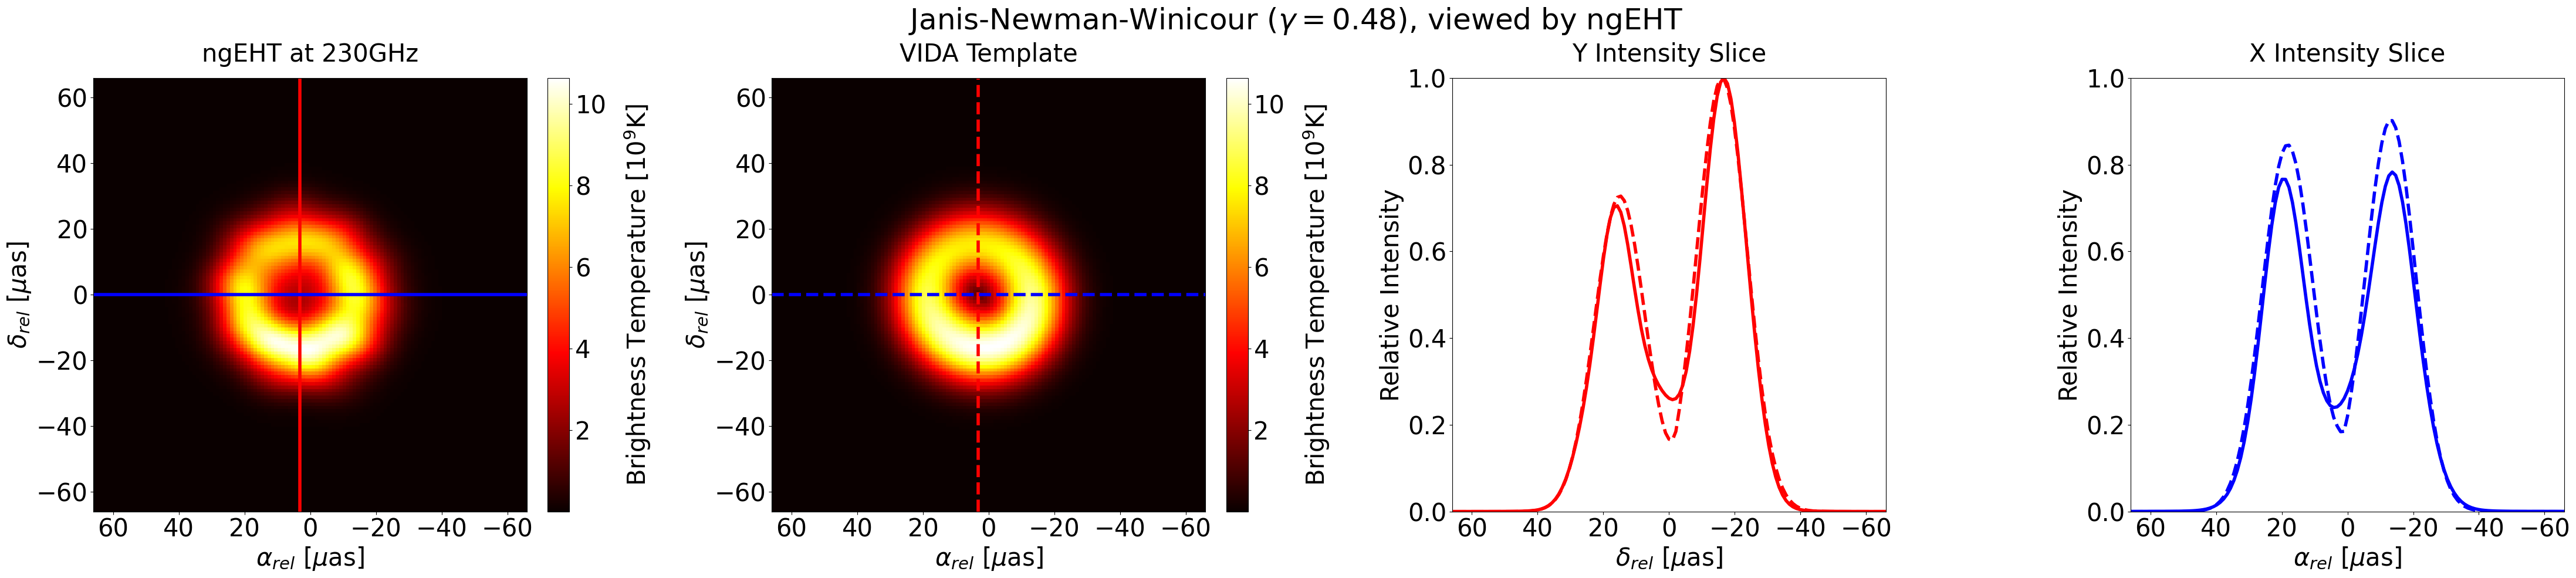
\includegraphics[scale = 0.13]{Ehtim_Vida_plot_ngEHT_230_JNW.png}
	\end{subfigure}\\
	\begin{subfigure}{12cm}
		\hspace{-1.5cm}
		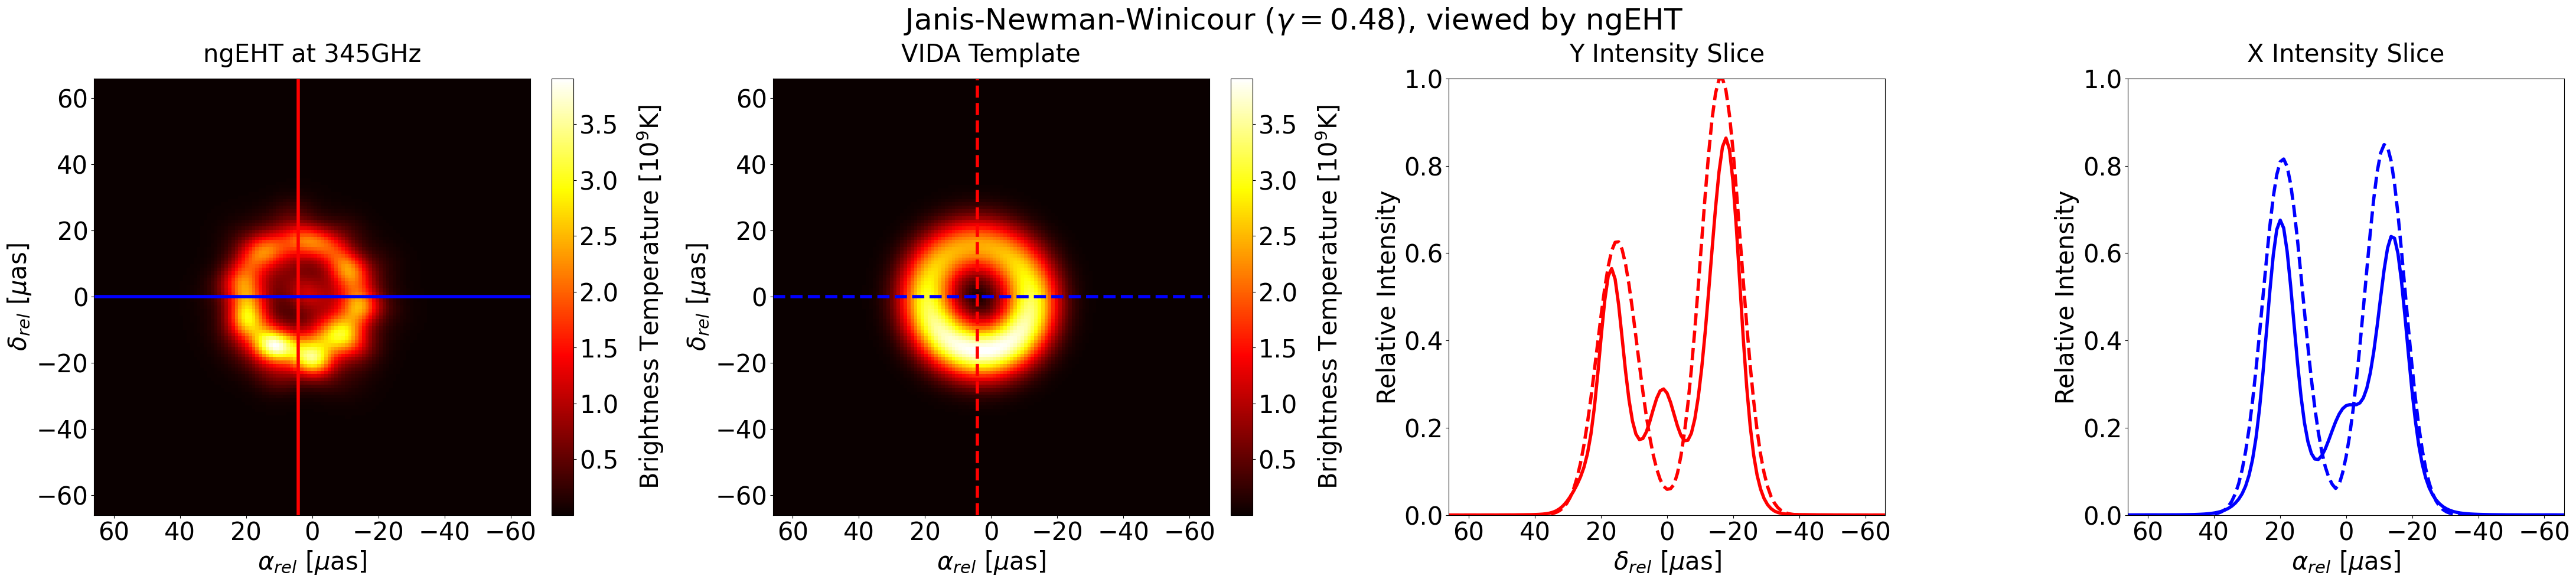
\includegraphics[scale = 0.13]{Ehtim_Vida_plot_ngEHT_345_JNW.png}
	\end{subfigure}\\
	\begin{subfigure}{12cm}
		\hspace{-1.5cm}
		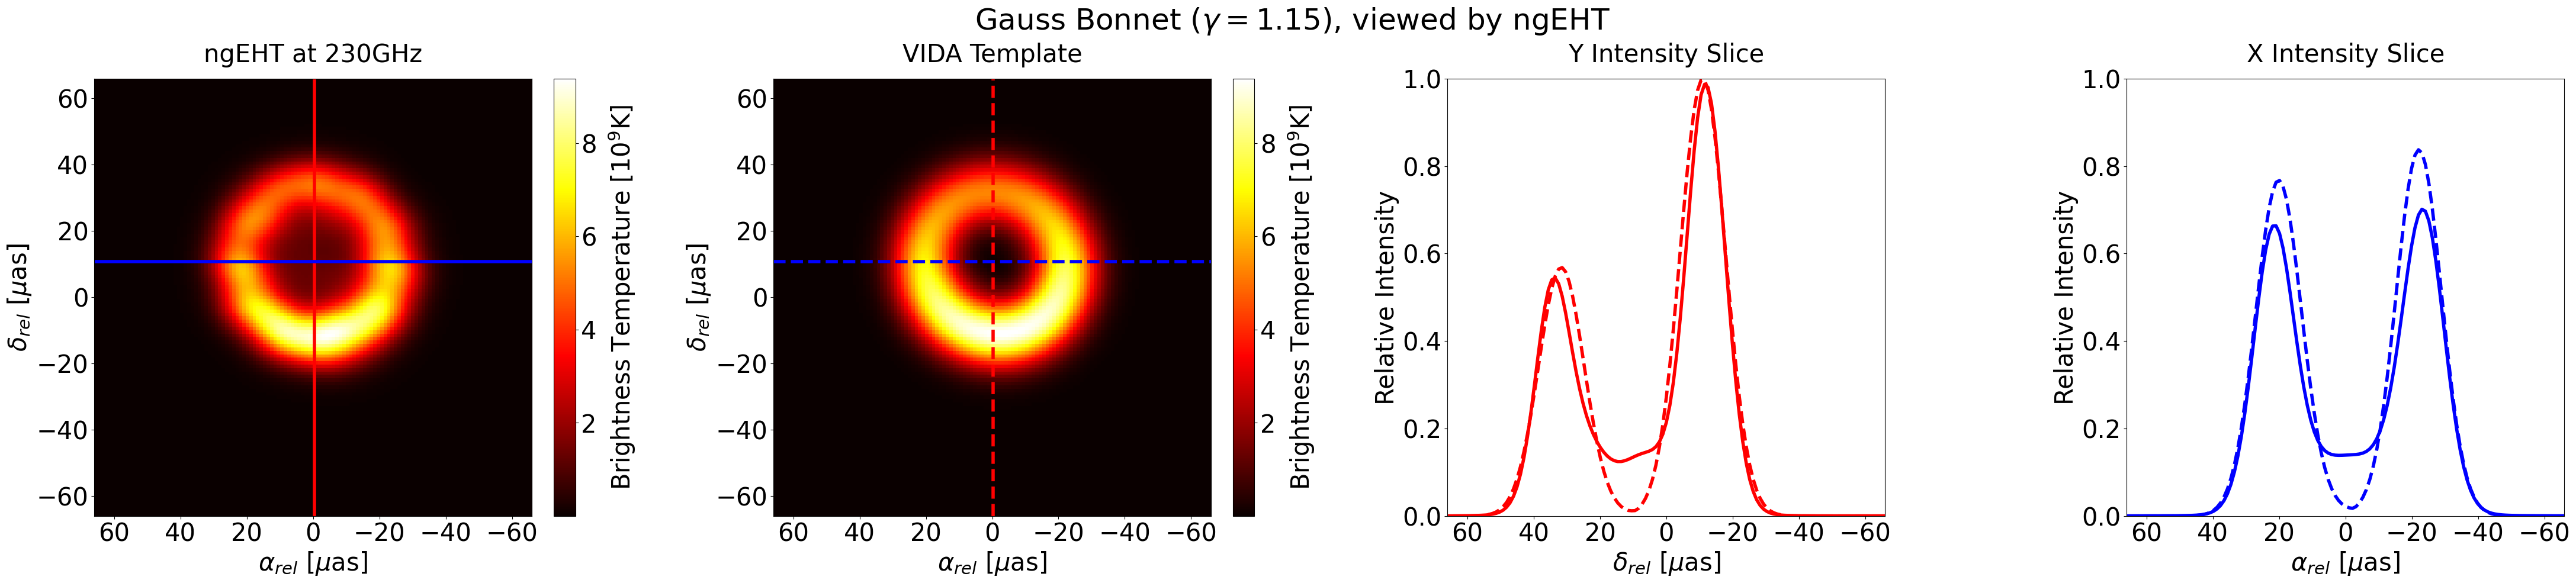
\includegraphics[scale = 0.13]{Ehtim_Vida_plot_ngEHT_230_GB.png}
	\end{subfigure}\\
	\begin{subfigure}{12cm}
		\hspace{-1.5cm}
		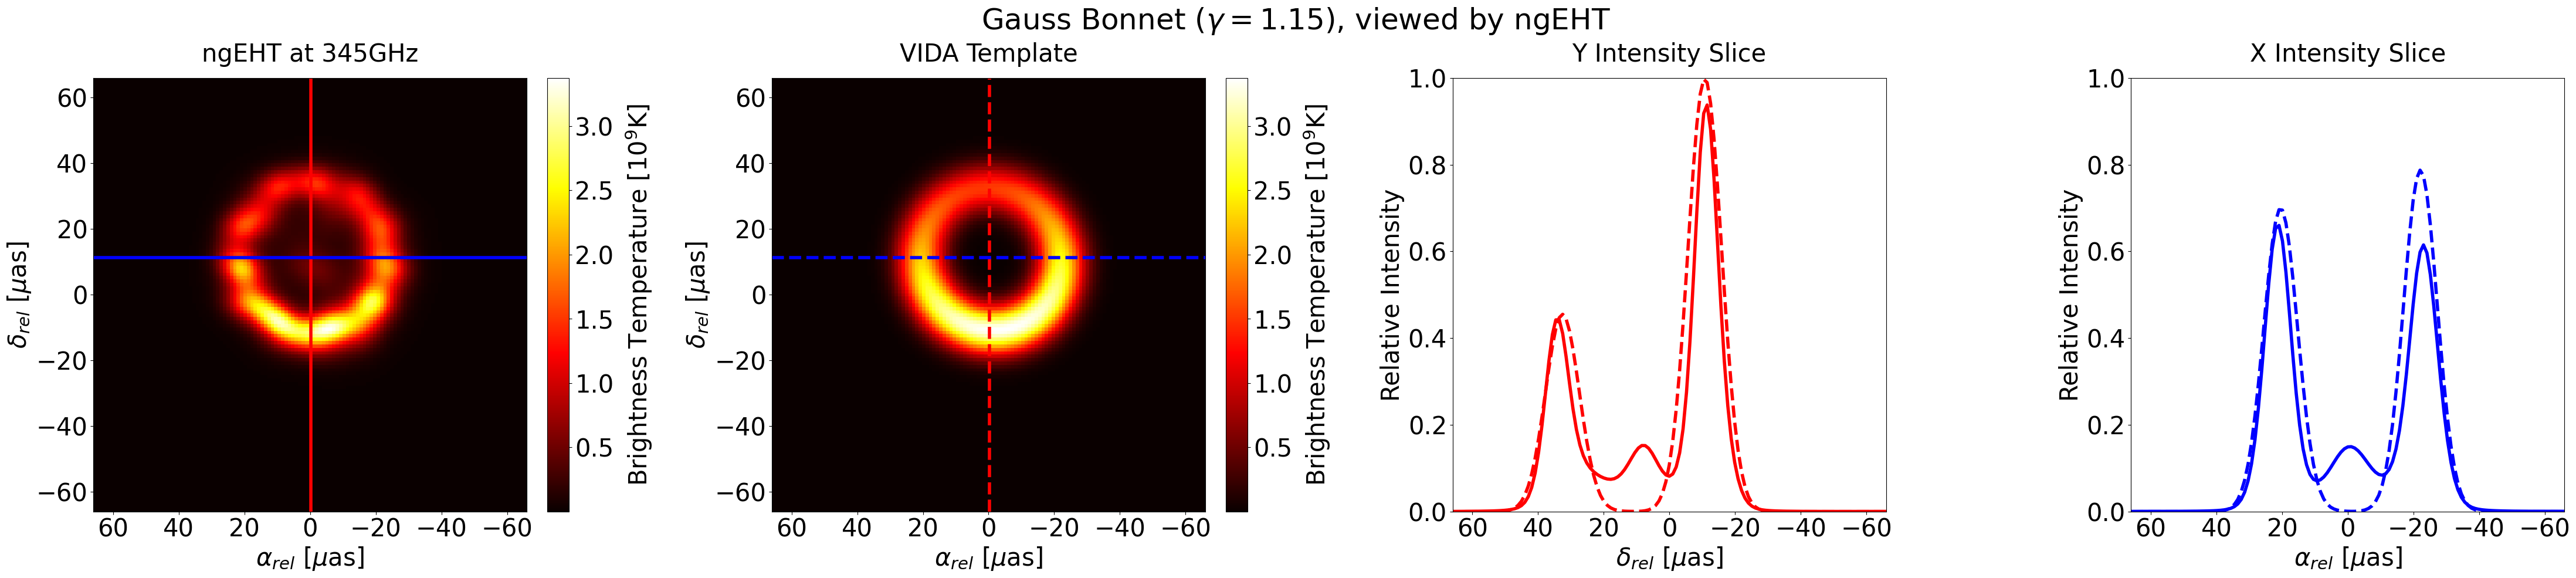
\includegraphics[scale = 0.13]{Ehtim_Vida_plot_ngEHT_345_GB.png}
	\end{subfigure}\\
	\label{VIDA_ngEHT_230}
	\caption[Темплейтен анализ на реконструкциите от ngEHT]{\small Темплейтен анализ на реконструкциите от ngEHT, за двете наблюдателни честоти $\nu = \{230, 345\}$ GHz. На десните два панела показваме профила на интензитета, и за двата образа, през центъра $(x_0,y_0)$ на темплейта.} 
\end{figure}

От друга страна, демонстрирахме, че добавянето на по-висока наблюдателна честота, заедно с увеличеното $(u,v)$ покритие на бъдещите конфигурации на телескопи, правят наблюденията чувствителни към централните екзотични образи. Разделителната способност не е достатъчно висока за да се отделят, или дори за да се съди за същинската им морфология, но реконструкциите показват ясен, и еднозначен централен максимум в депресията, който изцяло липсва при реконструкции на черни дупки на Кер. Показахме, че този максимум достига $30\%$ от максималният интензитет на целия образ, в случая за голи сингулярности на Джанис-Нюман-Уиникър, и до $15\%$ за Гаус-Боне. Показахме също, че количествената мярка за морфологията на централната депресия $\hat{f}_c$ се различава с два порядъка при новата наблюдателна честота $\nu = 345$  GHz.\\

С което заключваме, че въпреки неспособността на бъдещите наблюдения да отделят оптически релативистките образи на излъчващата среда един от друг, те могат да бъдат достатъчно чувствителни към екзотични образи, за да създадат ясна и еднозначна морфологична характеристика на реконструкциите - относително силен централен максимум, където бихме очаквали дълбока яркостна депресия. 

\begin{figure}[h!]
	\centering
	\begin{subfigure}{12cm}
		\hspace{-0cm}
		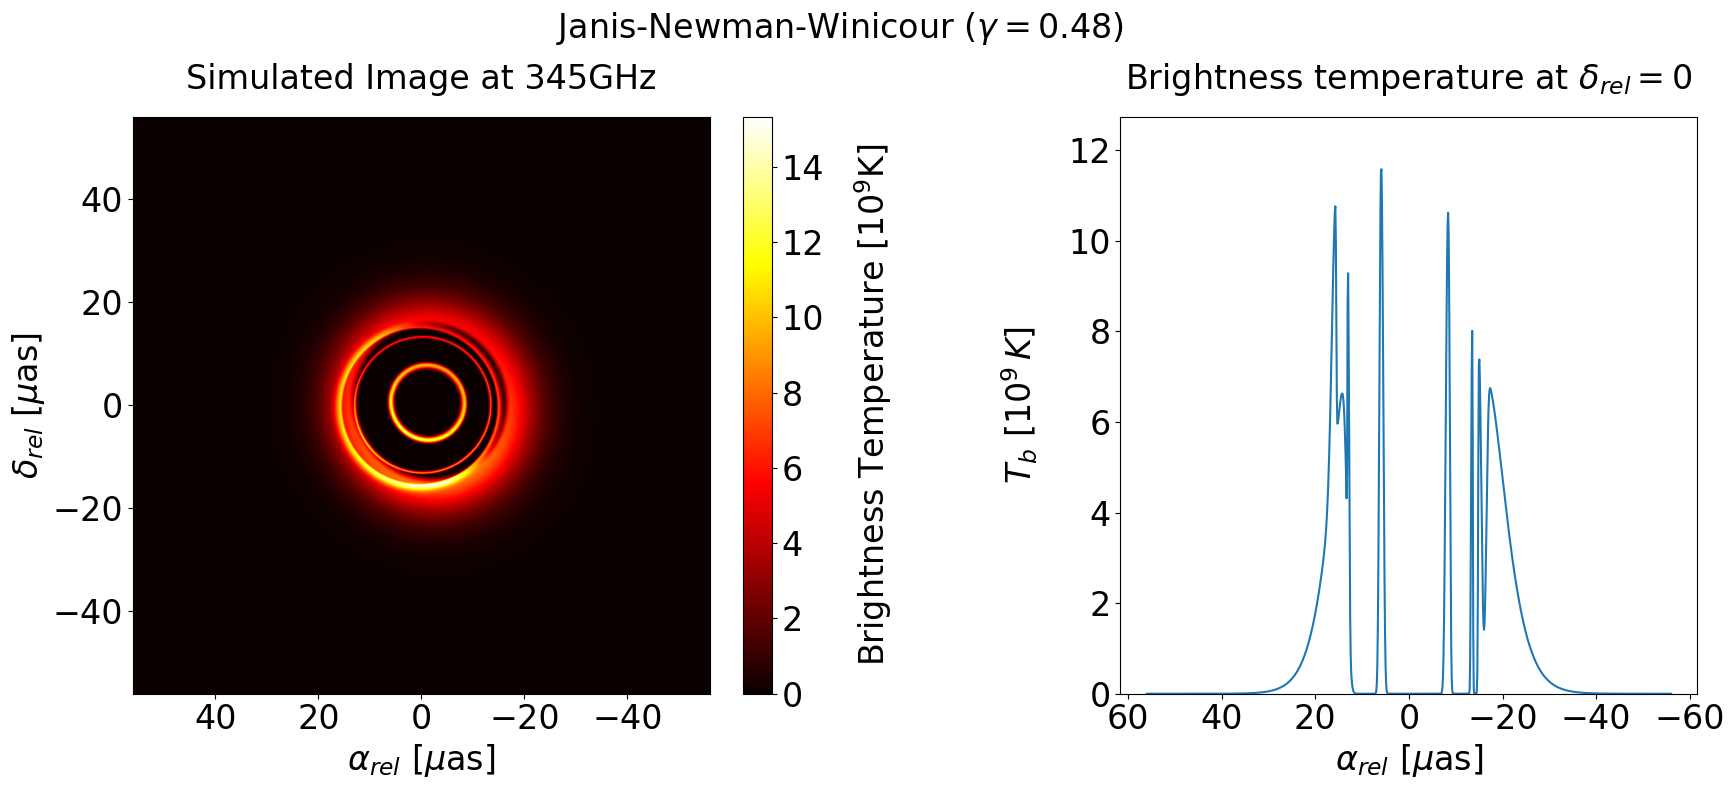
\includegraphics[scale = 0.25]{Ray_tracer_plot_345_JNW.png}
	\end{subfigure}\\
	\begin{subfigure}{12cm}
		\hspace{-0cm}
		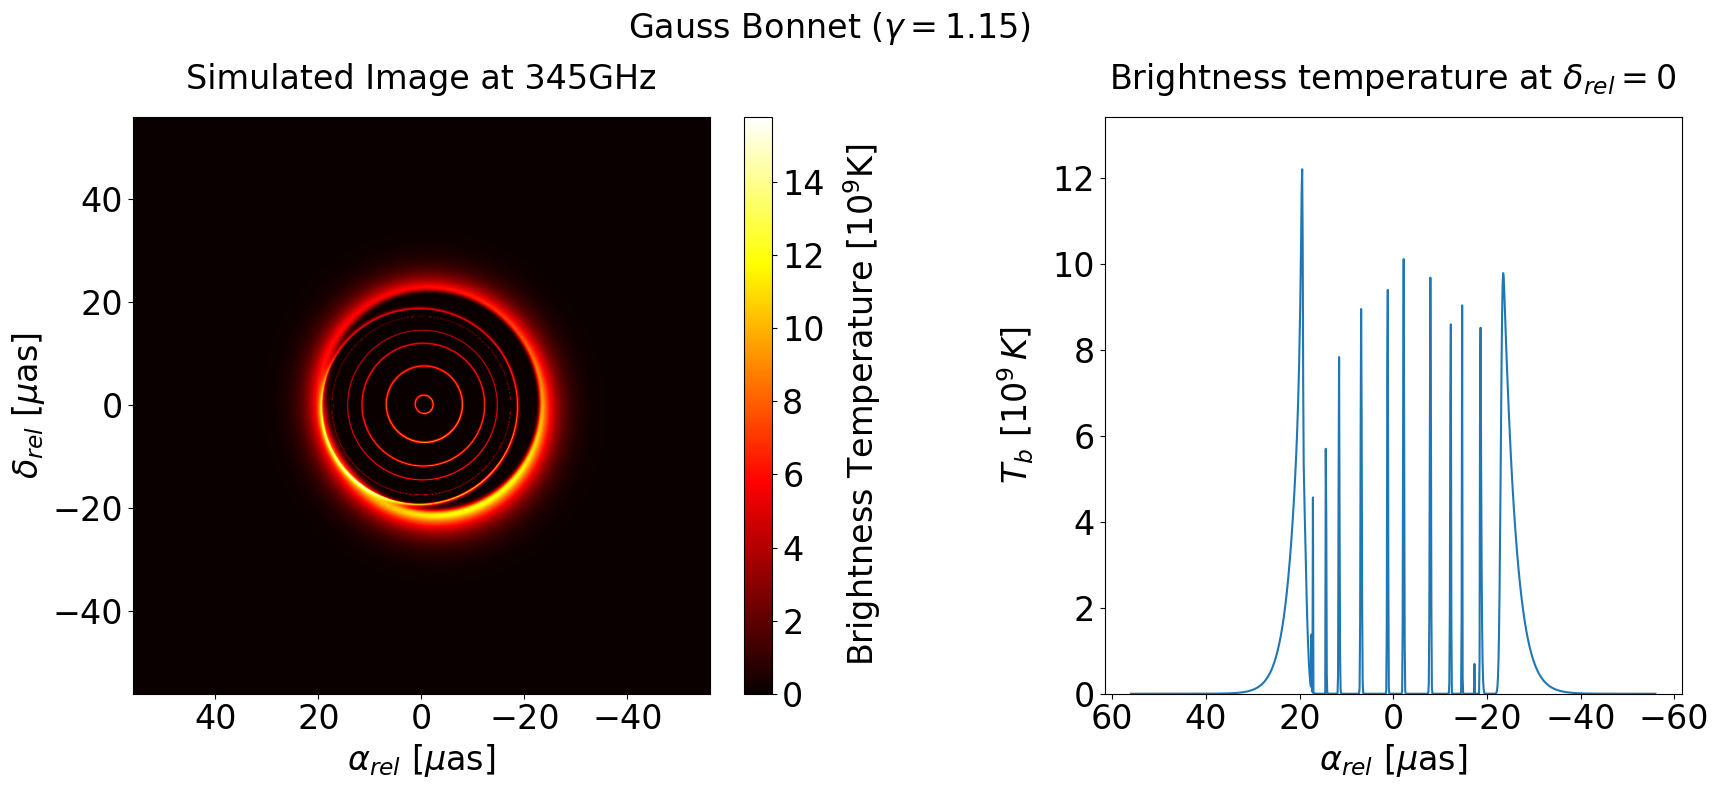
\includegraphics[scale = 0.25]{Ray_tracer_plot_345_GB.png}
	\end{subfigure}\\
	\label{Naked_Singularity_Ray_tracer_345}
	\caption[Идеални образи на голи сингулярности с реалистичен модел на излъчващата среда, при избрани стойности на $\gamma$ и $\nu_\text{obs} = 345$ GHz.]{\small Идеални образи на голи сингулярности с реалистичен модел на излъчващата среда, при избрани стойности на $\gamma$ и $\nu_\text{obs} = 345$ GHz. Температурата при $r = r_0,\,\,\theta = \frac{\pi}{2}$ за Джанис-Нюман-Уиникър е $T_0 = 7.2\times10^{10}$ K, докато за Гаус-Боне е $T_0 = 5.9\times10^{10}$. Пълният поток е съответно $\mathcal{F}_{\text{tot}} = 0.290$ Jy и $\mathcal{F}_{\text{tot}} = 0.262$ Jy. Параметърът $r_0$ е фиксиран на $r_0 = 5M$ за двете решения. За останалите параметри виж таблица \ref{table:Common_ray_tracer_params}.} 
\end{figure}